\documentclass[11pt]{article}
\usepackage[margin=1in]{geometry}
\usepackage[T1]{fontenc}
\usepackage{lmodern,amsmath,amssymb,amsthm,booktabs,array,longtable,graphicx}
\usepackage[colorlinks=true,linkcolor=blue,citecolor=blue,urlcolor=blue]{hyperref}
\usepackage{microtype}
\newtheorem{theorem}{Theorem}[section]
\newtheorem{lemma}[theorem]{Lemma}
\newtheorem{proposition}[theorem]{Proposition}
\newtheorem{corollary}[theorem]{Corollary}
\newtheorem{definition}[theorem]{Definition}
\newtheorem{remark}[theorem]{Remark}
\newcommand{\E}{\mathbb E}
\newcommand{\Pp}{\mathbb P}
\newcommand{\Prb}{\mathbb P}
\newcommand{\R}{\mathbb R}
\newcommand{\X}{\{-1,1\}^d}
\newcommand{\op}{\mathrm{op}}
\newcommand{\poly}{\operatorname{poly}}
\newcommand{\sgn}{\operatorname{sign}}
\title{A polynomial-depth learning bound for NNBayes on robust networks}
\author{Dmitry Vaintrob \and Kaarel H\"anni \and OpenAI Codex}
\date{18 October 2026}
\hypersetup{pdftitle={A polynomial-depth learning bound for NNBayes on robust networks},pdfauthor={Dmitry Vaintrob, Kaarel Hanni, OpenAI Codex}}
\begin{document}
\maketitle
\begin{abstract}
Can Bayesian neural networks learn small circuits with sample complexity
polynomial in circuit width and depth, independently of the
learner's width? For mean-field and stronger Gaussian prior scalings, this
remains open in general. We prove such a bound after restricting the prior
to networks whose
predictions are stable under a calibrated ball of simultaneous internal
perturbations. The networks are fully connected, with tanh activations and
a linear readout. For a Boolean target given by a layered circuit of width
$C$ and depth $H$, one polynomial bounds the required number of examples
jointly in input dimension, $C$, $H$, robustness calibration, and statistical
parameters. The guarantee holds simultaneously for learners with $H$ hidden
layers at every width $N\ge C$ and every Gaussian scale $0<t\le1$, including the
finite-variance mean-field scale and stronger priors. Training requires
exact label agreement with a fixed margin; the conclusion controls
posterior test error at a smaller margin and hence sign error. The proof
combines a robust implementation of each Boolean circuit with enough
Gaussian probability around it, posterior compression, and stability of
clipped predictions. We give the argument in full and separately assess
when trained networks satisfy the prior restriction.
\end{abstract}

\section{Introduction}

A function with a small circuit should be learnable from relatively few
examples, even by a neural network much larger than that circuit. For
Bayesian neural-network learning, or NNBayes, this asks whether conditioning
a prior on the training labels produces a posterior that predicts the
target well. A particularly useful guarantee would have sample complexity
polynomial in input dimension, target circuit width, and depth,
with no dependence on the learner's potentially much larger width.

The depth requirement is substantial. A bound polynomial in target width
at each fixed depth can still become exponential as depth grows. General
compression arguments for Gaussian neural-network priors incur such depth
costs because small errors introduced inside the network may be amplified
through successive layers. The full joint polynomial learning guarantee
remains open for Gaussian priors at mean-field and stronger-prior scalings
without an additional internal-stability restriction. Special target
classes permit better learner-depth bounds, but do not yet settle the case
of arbitrary small deep circuits.

This paper obtains a joint polynomial bound by restricting the prior.
We discard network parameterizations whose predictions are too sensitive
to small simultaneous disturbances of their internal activations. The
restriction concerns the computation performed by the network: changing
an internal value slightly should not substantially alter its prediction
score. We prove that every layered Boolean target circuit still has a
robust implementation with enough probability under the Gaussian prior.
Thus the restriction removes fragile implementations without requiring
the target function to be supplied with a robust neural implementation.

\paragraph{The learning guarantee.}
Consider a fully connected tanh network with $H=L-1$ hidden layers of
width $N$ and a real linear readout. The target is any Boolean function
on $d$ bits represented by a layered Boolean circuit of width $C$ and
at most $H$ stages; $C$ counts constant wires and any compilation or
padding needed for this representation. Inputs are sampled independently
from any fixed distribution. We start from independent Gaussian weights
with layer-dependent variances, restrict the prior by the stability
condition, and condition on signed training outputs greater than $1/2$.
For a fixed stability calibration $c>0$, a sufficient sample size is
\[
 n\ge\operatorname{poly}
       \bigl(d,L,C,c+c^{-1},\varepsilon^{-1},\log(1/\delta)\bigr).
\]
With probability at least $1-\delta$ over the sample, the posterior's
average probability of a signed test output at most $1/4$ is then at
most $\varepsilon$. The polynomial degree does not grow with depth.
One sample event gives this guarantee for every $N\ge C$ and every
Gaussian scale $0<t\le1$ in the model of Section~\ref{sec:theory-model}.
In the exponent convention $t=N^{(1-\gamma)/2}$, this includes
$\gamma=1$ at finite width as well as every $\gamma>1$; no width or
small-variance limit is needed.

The conclusion controls sign error and posterior confidence as well as
this test-margin loss. For example, the test-distribution mass of inputs at which
the posterior assigns probability at most $2/3$ to the correct sign is
at most $3\varepsilon$. The guarantee concerns exact Bayesian conditioning;
it does not supply an efficient posterior-sampling algorithm.

\paragraph{What the restriction requires.}
We clip the output at the training margin, obtaining a score in
$[-1/2,1/2]$. At every Boolean input, this score must change by at most
$1/16$ under every simultaneous internal and output disturbance in a
specified ball. Its radius is calibrated by depth and readout energy,
as defined in Section~\ref{sec:theory-model}. Clipping makes the condition
insensitive to large changes between already confident outputs of the
same sign: a change from $10$ to $1$ leaves the score unchanged. The
condition also permits small clean outputs at unobserved inputs; the
learning argument, rather than an all-input margin assumption, makes
weak or incorrect test predictions rare. This is a learning theorem
under a robustness restriction, not a claim that every trained network
satisfies that restriction.

\paragraph{Why the proof gives polynomial depth.}
First, we implement the target circuit robustly at every width $N\ge C$
and bound the Gaussian probability of a neighborhood of that
implementation. This bounds the posterior's relative entropy with
respect to the original Gaussian. Second, an entropy-compression argument
constructs a distribution on one finite candidate class shared by all
widths and scales. At each input, the candidate and posterior computations
can be coupled through small internal disturbances, with the same
marginal distributions at every input. The support restriction then
controls the prediction error directly, without multiplying
worst-case amplification factors across layers. Finally, a uniform
sampling bound for that finite class transfers training fit to test
accuracy. The result is polynomial jointly in depth and the other
parameters, although the polynomial is too loose to provide practical
sample estimates.

\paragraph{Relation to prior work and verification.}
Compression through noise stability and all-layer margins has precedents
in work of Arora et al.\ and Wei and Ma~\cite{arora,weima}.
Wei, Chen, and Ma~\cite{weichenma} prove polynomial circuit-size sample
bounds for overparameterized feedforward networks using a suitable
all-layer-margin surrogate and robust circuit simulation. The role of
robust simulation in avoiding exponential depth factors therefore
predates this paper. Here we analyze the posterior of a specified
Gaussian prior, including its target probability and a single learning
guarantee uniform over widths and finite Gaussian scales.
A companion Lean development verifies the qualitative main learning
theorem for the exact robust-only posterior, using a looser polynomial
from a Pinsker-and-energy construction. It does not certify every
quantitative constant, extension, or empirical certificate in this paper.

\paragraph{Organization.}
Section~\ref{sec:theory-model} specifies the prior and loss, and
Section~\ref{sec:theory-main} states the theorem.
Sections~\ref{sec:theory-statistical} and~\ref{sec:theory-target-cylinder}
give the statistical argument and robust target construction;
Appendix~\ref{sec:robust-entropy} supplies the full compression proof.
Section~\ref{sec:restriction-in-practice} discusses the meaning of the
restriction for trained networks. The remaining appendices give
certificates, weaker and localized restrictions, and the detailed
empirical evidence. The main result and its proof can be read without
any companion paper.

\section{Model, prediction convention, and stability restriction}
\label{sec:theory-model}

Let $\mathcal X=\{-1,1\}^d$, let $D$ be any distribution on $\mathcal X$,
and let $f:\mathcal X\to\{-1,1\}$ be the target. A network has $H=L-1$
hidden layers, each of width $N$, tanh activations, and a linear readout:
\[
 h^1=\tanh(W^1\bar x),\qquad
 h^s=\tanh(W^s h^{s-1})\ (2\le s\le H),\qquad
 z_w(x)=v^\top h^H,
 \qquad \bar x=(x,1).
\]
The first layer includes a bias coordinate; internal constants are carried
by ordinary hidden wires. Let $\mu_{N,t}$ be the product Gaussian with entry
variances $t^2/d$ in $W^1$, $t^2/N$ in the internal matrices, and $t^2/N^2$
in $v$, where $0<t\le1$. The exponent convention
$t=N^{(1-\gamma)/2}$ therefore gives every $\gamma\ge1$. Define
\[
 \kappa_N(w)=\frac dN\|W^1\|_F^2+
           \sum_{s=2}^H\|W^s\|_F^2+N\|v\|^2,
 \qquad E_v(w)=N\|v\|^2.
\]
In these energy coordinates the Gaussian density is proportional to
$\exp[-N\kappa_N/(2t^2)]$.

A disturbance is added after every hidden activation and at the readout:
\[
 h^1_\eta=\tanh(W^1\bar x)+\eta^1,\qquad
 h^s_\eta=\tanh(W^s h^{s-1}_\eta)+\eta^s,\qquad
 z_w(x;\eta)=v^\top h^H_\eta+\eta^{\rm out}.
\]
The simultaneous disturbance budget is
\begin{equation}\label{eq:standalone-noise}
 \|\eta\|_*^2=\sum_{s=1}^H\frac{\|\eta^s\|_2^2}{N}
                       +|\eta^{\rm out}|^2.
\end{equation}
This is an adversarial finite perturbation, not a Gaussian-noise average or
a derivative evaluated only at the clean computation. Noisy hidden states
need not stay in $[-1,1]^N$.

Our training likelihood is
\begin{equation}\label{eq:standalone-likelihood}
 \mathcal L_S(w)=\prod_{i=1}^n
       \mathbf1\{f(X_i)z_w(X_i)>1/2\}.
\end{equation}
At test time we count $f(x)z_w(x)\le1/4$ as an error. This stronger loss
also bounds sign error. There is no requirement that unobserved inputs have
any clean output margin.

Clip the output at the training margin:
\[
 T(u)=\max\{-1/2,\min\{1/2,u\}\}.
\]
For a calibration parameter $c>0$, set
\begin{equation}\label{eq:standalone-radius}
 r_c(w)=\frac{c}{\sqrt{1+H E_v(w)}}.
\end{equation}
Let $\mathcal R_{N,c}$ be the set of networks satisfying
\begin{equation}\label{eq:standalone-support}
 |T(z_w(x;\eta))-T(z_w(x))|\le1/16
 \quad\text{for every }x\in\mathcal X
 \text{ and every }\|\eta\|_*\le r_c(w).
\end{equation}
The prior is exactly $\mu_{N,t}$ conditioned on $\mathcal R_{N,c}$.
The posterior $Q_{S,N,t,c}$ additionally conditions on
\eqref{eq:standalone-likelihood}. Both conditioning events have positive
probability by the target construction below. No tractable sampling
algorithm is assumed or supplied by the theorem.

The clipping scale is set by the existing likelihood convention. For
example, changing a raw output from $10$ to $1$ causes no score change.
Clipping at $\pm1/2$ gives a weaker condition than clipping at $\pm1$ with
the same tolerance and noise radius, because
$T=T\circ T_1$, where $T_1$ clips at $\pm1$, and $T$ is $1$-Lipschitz.

\section{The learning theorem}
\label{sec:theory-main}

A width-$C$, depth-$H$ layered Boolean circuit has at most $C$ Boolean wires
at each of its $H$ stages. We use NAND gates, copies, and negations;
constant wires required by internal gate implementations are carried
through the circuit and count toward $C$. This is a universal Boolean
basis. Compiling another fixed basis into this one may change the width
and depth, and those resources must be counted. Its output is one final wire.
The circuit's logical depth must fit the $H$ hidden layers; idle stages
can be filled with copies.

\begin{theorem}[Polynomial depth at every width and every $\gamma\ge1$]
\label{thm:standalone-clipped}
There is a universal polynomial $P$ with the following property. Let $f$
be computed by such a width-$C$, depth-$H$ Boolean circuit, and let $D$ be
any input distribution. For every $c>0$ and every $0<\varepsilon,\delta<1$, if
\[
 n\ge P\bigl(d,L,C,c+c^{-1},\varepsilon^{-1},\log(1/\delta)\bigr),
\]
then with probability at least $1-\delta$ over the iid labeled sample,
\begin{equation}\label{eq:standalone-risk}
 \mathbb E_{w\sim Q_{S,N,t,c},\,X\sim D}
       \mathbf1\{f(X)z_w(X)\le1/4\}\le\varepsilon
\end{equation}
simultaneously for every $N\ge C$ and $0<t\le1$.
The polynomial degree is independent of width, depth, and Gaussian scale.
In particular, the result includes the actual finite-variance mean-field
scale $\gamma=1$ and every stronger-prior scale $\gamma>1$.
\end{theorem}

The same theorem holds if the prior is additionally conditioned on
$|z_w(x)|>1/2$ at every input, as in the original globally margin-conditioned
model. This variant is argued here; it is not part of the Lean-checked
statement, which concerns the robust-only posterior. The target cylinder constructed below already satisfies this extra
condition. Its probability bound and every subsequent statistical step are
therefore unchanged. Under that additional condition, test-margin error
coincides with sign error. Dropping the extra condition is permitted, but is
not required for the result.

The width threshold concerns a layered Boolean circuit, not an arbitrary
real-valued neural-network representation of the same Boolean function.
The theorem does not assert that every function with a small real neural
circuit has a comparably small Boolean circuit at the same depth, or that
all its low-energy neural representations satisfy the stability condition.
The proof instead supplies one robust implementation of each Boolean
circuit, together with enough Gaussian probability around that implementation.

Define the posterior correct-margin probability
$p_S(x)=Q_{S,N,t,c}\{f(x)z_w(x)>1/4\}$.
Equation~\eqref{eq:standalone-risk} immediately implies
\[
 D\{x:p_S(x)\le2/3\}\le3\varepsilon,
 \qquad D\{x:p_S(x)\le1/2\}\le2\varepsilon.
\]
The same bounds hold for posterior sign correctness, since the correct-sign
event contains the correct-margin event. These conclusions allow arbitrary
posterior mixtures; they do not require concentration on one predictor.

\section{Compression and the statistical proof}
\label{sec:theory-statistical}

The constructive compression statement needed here concerns numerical
outputs before any robustness condition is used.

\begin{lemma}[Entropy compression before the prediction comparison]
\label{lem:raw-entropy-compression}
For $d\ge1$, $L\ge2$, $K\ge1$, $0<r\le1$, and
$0<\alpha\le1/8$, there is a finite class $\mathcal H$ of real-valued
bounded-weight depth-$L$ tanh networks, independent of $N,t$, such that
\[
 \log|\mathcal H|\le
       \operatorname{poly}(d,L,K,r^{-1},\alpha^{-1}).
\]
If $Q\ll\mu_{N,t}$ satisfies
$D_{\rm KL}(Q\Vert\mu_{N,t})\le NK/t^2$, there is one distribution
$\Gamma_Q$ on $\mathcal H$ with the following property. For every fixed
$x$, one can couple $w\sim Q$ and $h\sim\Gamma_Q$ so that, except with
probability at most $\alpha$, there is a disturbance $\eta$ with
\[
 \|\eta\|_*<r/2,\qquad
 |h(x)-z_w(x;\eta)|\le r/8.
\]
The couplings and disturbances may depend on $x$, but their two marginals
are the same at every input. No robustness or clean-margin assumption is
made on $Q$.
\end{lemma}

The proof is constructive: it retains a bounded number of input directions
carrying conditional Gaussian relative entropy in each layer, replaces the
remaining directions by Gaussian randomness, samples a bounded number of
source neurons, and rounds a bounded-size network to a fixed grid.
The resulting virtual computation is the original network under small
postactivation disturbances. The appendix gives the complete construction;
the prediction comparison below is the first step that uses stability.

\begin{lemma}[Readout truncation]
\label{lem:standalone-readout-tail}
Suppose a posterior is the raw Gaussian conditioned on an event of mass at
least $\exp(-ND_*/t^2)$, where $D_*\ge1$. For $0<\beta\le1/2$, put
\[
 B=\max\{8,8[D_*+\log(1/\beta)]\}.
\]
It assigns mass at most $\beta$ to $E_v>B$. Its conditional law $Q'$ on
$E_v\le B$ satisfies
$D_{\rm KL}(Q'\Vert\mu_{N,t})\le N(D_*+1)/t^2$.
\end{lemma}
\begin{proof}
Under the Gaussian, $NE_v/t^2$ has the chi-square distribution with $N$
degrees of freedom. Its exponential moment gives, for $B\ge8$,
\[
 \mu_{N,t}\{E_v>B\}
 \le e^{-NB/(4t^2)}2^{N/2}
 \le e^{-NB/(8t^2)}.
\]
Divide by the conditioning-event probability and use $N/t^2\ge1$.
The further conditioning event has raw probability at least
$(1-\beta)e^{-ND_*/t^2}$, so its negative logarithm is at most
$ND_*/t^2+\log[1/(1-\beta)]\le N(D_*+1)/t^2$.
\end{proof}

\begin{proof}[Statistical proof of Theorem~\ref{thm:standalone-clipped}]
The next section constructs a subset of the support with correct noisy
margin on every input and raw mass at least $e^{-ND_*/t^2}$, where
$D_*=\operatorname{poly}(d,L,C,c)$ is independent of $N,t$.
It is contained in the posterior conditioning event for every correctly
labeled sample. Apply Lemma~\ref{lem:standalone-readout-tail} with
$\beta=\varepsilon/4$, and write $Q'$ for the retained law. Set
\[
 K=D_*+1,\qquad
 r=\min\{1/6,c/\sqrt{1+HB}\},\qquad
 \alpha=\varepsilon/12.
\]
Every retained network satisfies the score-stability condition at the common
radius $r$. Lemma~\ref{lem:raw-entropy-compression} and the $1$-Lipschitz
property of $T$ therefore give pointwise couplings with
\[
 \Pr\{|T(h(x))-T(z_w(x))|>1/12\}\le\alpha,
\]
because $1/16+r/8\le1/12$.

Use the bounded ramp loss
\[
 \psi(u)=
 \begin{cases}
 1,&u\le1/3,\\
 5-12u,&1/3<u<5/12,\\
 0,&u\ge5/12.
 \end{cases}
\]
At a training input, $f(x)z_w(x)>1/2$ implies $f(x)T(z_w(x))=1/2$.
A successful coupling therefore gives $f(x)T(h(x))\ge5/12$, so its ramp
loss is zero. The candidate's averaged empirical ramp risk is at most
$\alpha$. At a test input with $f(x)z_w(x)\le1/4$, a successful coupling
gives $f(x)T(h(x))\le1/3$, so its ramp loss is one.

For any finite class of $[0,1]$-valued losses, a relative Chernoff bound
and a union bound give, with probability at least $1-\delta$,
\[
 \mathbb E_D\psi(f(X)T(h(X)))
 \le\frac2n\sum_{i=1}^n\psi(f(X_i)T(h(X_i)))
       +\frac{8[\log|\mathcal H|+\log(1/\delta)]}{n}
 \quad(h\in\mathcal H).
\]
For completeness, $e^{-u}\le1-(1-e^{-1})u$ on $[0,1]$ gives the usual
lower-tail exponent at least the mean divided by eight. This proves the
displayed bound for one loss, and a union bound proves simultaneity.
Average under the sample-dependent law $\Gamma_{Q'}$, apply the population
comparison, and restore the discarded posterior mass. The result is
\[
 \Pr_{Q_{S,N,t,c},D}\{f(X)z_w(X)\le1/4\}
 \le\beta+3\alpha+
       \frac{8[\log|\mathcal H|+\log(1/\delta)]}{n}.
\]
Choose $n$ so the last term is at most $\varepsilon/2$.
Every quantity entering $\log|\mathcal H|$ is bounded by a universal
polynomial in the theorem's parameters. Its class and the displayed sample
event are independent of $N,t$, establishing the simultaneous statement.
\end{proof}

\section{A robust target cylinder at every width}
\label{sec:theory-target-cylinder}

We give the probability bound used in the statistical proof. It uses a
robust digital implementation, not a claim that every implementation is
stable. Let $N\ge C$. Partition the neurons into $C$ balanced clone groups
of sizes $k_a\in\{\lfloor N/C\rfloor,\lceil N/C\rceil\}$, so
$C/2\le N/k_a\le2C$. Let $P$ project onto vectors constant on each clone
group. Fill unused logical slots with available constants or copies of an
existing Boolean wire. The ideal wire
vector $b^s(x)$ then has entries in $\{-1,1\}$, belongs to the range of
$P$, and has Euclidean norm $\sqrt N$.

Use gain $A$ in the tanh simulation of every Boolean gate. For example,
NAND on $u,v\in\{-1,1\}$ is the sign of $1-u-v$; copies and negations
use $u$ and $-u$. Bias constants in internal layers are supplied by counted
constant wires. The ideal signed preactivation of every gate is at least
$A$. In the clone implementation, each coefficient from a logical wire is
divided equally among that wire's clones. Set
\begin{align*}
 e_*&=\frac1{16\sqrt{2C}},&
 \tau_0&=\frac{e_*}{4},&
 b_L&=\sqrt{16\log9+8\log(4L)},\\
 A&=\max\{32b_L,2\log(8/e_*)\},&
 a&=\max\{2,256c\},&
 \rho&=\min\{1/4,A/[4(d+1)],Ae_*/(64\sqrt C)\}.
\end{align*}
The teacher readout averages the clones of the output wire with total
coefficient $a$.

In Gaussian coordinates $\sqrt d\,W^1$, $\sqrt N\,W^s$, and $Nv$, all
entries have variance $t^2$. Restrict each first-layer coordinate, each
internal row's projection onto every normalized clone-group direction, and
each readout coordinate to an interval of radius $\rho t$ about its teacher
value. The internal matrices then decompose as
\[
 W^s=W_*^s+R^s+E^s,\qquad
 R^s=R^sP,\quad \|R^s\|_{\rm op}\le\rho t\sqrt C,
 \quad E^sP=0.
\]
The remaining Gaussian bulk $E^s$ is independent of the constrained
coordinates. A $1/4$-net of the unit sphere has at most $9^N$ points,
and the usual two-net Gaussian bound gives
\[
 \Pr\{\|E^s\|_{\rm op}>b_Lt\}
 \le2\exp(2N\log9-Nb_L^2/8)\le\frac1{2L}.
\]
Thus all bulk norms are at most $b_Lt$ with conditional probability at
least $1/2$.

\paragraph{Finite disturbance robustness.}
Allow a separate RMS disturbance of size $\tau_0$ at each hidden layer and
scalar output disturbance at most $\tau_0$. This includes the entire
total-budget ball $\|\eta\|_*\le\tau_0$.
Write $e_s=\|h^s_\eta-b^s\|_2/\sqrt N$.
If $e_{s-1}\le e_*$, every clone-group mean differs from its ideal bit by
at most $e_*\sqrt{N/k_a}\le1/16$. At most three teacher coefficients,
including a constant coefficient, enter a gate, so its intended signed
preactivation remains at least $A/2$.
For $\epsilon\in\{-1,1\}$ and real $u$, the elementary global secant bound
\[
 \epsilon q\ge A/2
 \quad\Longrightarrow\quad
 |\tanh(q+u)-\epsilon|\le2e^{-A/2}+8|u|/A
\]
holds: for $|u|<A/4$ use saturation, and otherwise the linear term is at
least two. Since $E^sb^{s-1}=0$ and
$\|h^{s-1}_\eta\|_2/\sqrt N\le1+\tau_0$, it follows that
\[
 e_s\le2e^{-A/2}+
          (8/A)\rho\sqrt C(1+\tau_0)
          +(8b_L/A)e_{s-1}+\tau_0\le e_*.
\]
Each of the four terms is at most $e_*/4$.
The first layer initializes the same invariant: its coordinatewise
preactivation perturbation is at most $\rho(d+1)\le A/4$, and its
postactivation disturbance contributes at most $\tau_0$ in RMS norm.
Consequently the noisy signed readout is at least
\[
 f(x)z_w(x;\eta)
 \ge\frac{15a}{16}-\rho(1+\tau_0)-\tau_0>1
 \qquad(x\in\mathcal X,\ \|\eta\|_*\le\tau_0).
\]

The readout center satisfies $\sqrt N\|v_*\|\ge a\sqrt{C/2}$, and its
permitted perturbation has $\sqrt N\|v-v_*\|\le\rho$.
Therefore $E_v\ge a^2C/8$, whence
\[
 r_c(w)\le\frac{2\sqrt2c}{a\sqrt C}
       \le\frac1{64\sqrt{2C}}=\tau_0.
\]
All clean and noisy clipped scores on the calibrated ball equal $f(x)/2$.
The entire cylinder, with the bulk-norm event imposed, therefore belongs
to $\mathcal R_{N,c}$ and satisfies the training likelihood for every sample.
This also proves why every fixed $c>0$ is allowed: a larger calibration
requires only a polynomially larger readout coefficient.

\paragraph{Gaussian mass.}
There are $Nq$ constrained independent scalar coordinates, where
$q=d+2+(L-2)C$. The sum of their squared centers is at most $NB_0$, with
\[
 B_0=9dA^2+18(L-2)CA^2+2a^2C.
\]
These loose constants cover the fan-in-two gate implementation above.
For $Z\sim\mathcal N(0,t^2)$, $\rho\le1/4$, and any center $m$,
\[
 \Pr\{|Z-m|\le\rho t\}
 \ge\frac{2\rho}{e\sqrt{2\pi}}\exp(-m^2/t^2).
\]
Multiplication over the coordinates and the independent bulk event gives
\begin{equation}\label{eq:standalone-cylinder-mass}
 \mu_{N,t}(\text{target cylinder})
 \ge\exp(-ND_*/t^2),\qquad
 D_*=B_0+q\log\frac{e\sqrt{2\pi}}{2\rho}+\log2.
\end{equation}
Here $D_*\ge1$ and is bounded by a universal polynomial in $d,L,C,c$.
The construction and estimate hold at every integer width $N\ge C$.


\section{What the restriction means for trained networks}
\label{sec:restriction-in-practice}

The theorem's prior restriction is motivated by stability of a computation,
but its empirical relevance is a separate question. It quantifies over
every Boolean input and every allowed finite disturbance. Stability to
random noise on a test set is useful evidence, but has different
quantifiers. Published experiments report attenuation of injected
activation noise in a VGG-19 trained on CIFAR-10~\cite{arora}, and improved
noise stability in residual networks relative to matched plain
networks~\cite{yutomasi}. They do not establish the support condition
used here.

There are concrete sufficient conditions. If every internal hidden-layer
map is nonexpansive, meaning it does not increase Euclidean distances,
then the readout-and-depth calibration makes the required bound hold
for $c\le1/16$. Individual layers need not all be nonexpansive: bounds
on their combined effects, or saturation of tanh along the reachable
computations, can also certify stability.
Appendix~\ref{sec:standalone-stability-certificates} develops these tests.
A calibration $c$ that decreases only polynomially with depth still gives
a polynomial sample bound.

Our experiments and exact-arithmetic certificates give mixed evidence.
Some image classifiers fitted to every training label satisfy a global
stability certificate at the stated small calibrations, and two trained
64-hidden-layer Boolean classifiers satisfy the condition on their entire
finite input domains. Another fitted image model has a verified
confident-input counterexample even though it satisfies certificates
on all 10,000 official held-out images at the same radius.
The experiments, domain conventions, and certificate scopes are reported
in Appendices~\ref{sec:empirical-interpretation},
\ref{sec:image-experiments}, and~\ref{sec:verified-trained-networks}.
In particular, a certificate at one input covers that input only, and
failure to find an adversarial disturbance is not a certificate.

Gradient descent does not automatically enforce the condition:
Appendix~\ref{sec:analytic-gd-counterexample} gives an exact construction
that is stable on the data distribution and fragile elsewhere.
Localized versions of the prior can allow exceptional input regions when
their complexity is controlled (Appendix~\ref{sec:localized-prior-theorem}).
Whether the global condition, or such a localized version, commonly holds
for relevant trained networks remains a substantive empirical question.
These investigations concern membership in the restricted prior;
they do not identify the distribution of gradient-descent outputs with
the Bayesian posterior analyzed by the theorem.

\clearpage
\appendix
\section{Finite posterior compression by internal-noise coupling}
\label{sec:robust-entropy}

This appendix gives the compression construction used in the main theorem.
It tracks relative entropy only in the original weights that have not yet
been processed. The compressed prefix need not have a Gaussian density.
No stability assumption is needed until the coupling is used in the main
statistical argument.

\begin{theorem}[Finite compression before invoking stability]
\label{thm:robust-entropy}
Fix a scalar $1$-Lipschitz activation $|\phi|\le1$, and parameters
$d\ge1$, $L\ge2$, $K\ge1$, $0<r\le1$, and $0<\alpha\le1/8$.
There is a finite class $\mathcal H=\mathcal H(d,L,K,r,\alpha)$ of
real-valued bounded-weight depth-$L$ network outputs with
\[
 \log|\mathcal H|\le\poly(d,L,K,r^{-1},\alpha^{-1}).
\]
The polynomial and class are independent of width $N$ and scale $0<t\le1$.
For every $Q\ll\mu_{N,t}$ with
$D_{\rm KL}(Q\Vert\mu_{N,t})\le NK/t^2$, there is a law $\Gamma_Q$ on
$\mathcal H$ such that, at every Boolean input $x$, one can couple
$w\sim Q$, $h\sim\Gamma_Q$, and a disturbance $\eta$ so that
\[
 \Prb\left\{\|\eta\|_*<r/2,\quad
       |h(x)-z_w(x;\eta)|\le r/8\right\}\ge1-\alpha.
\]
The coupling may depend on $x$; its two specified marginals do not.
\end{theorem}

We give the proof, including deliberately loose polynomial choices.
Two elementary entropy facts organize the construction. First, for a standard
$D$-dimensional Gaussian $G$, the entropy variational inequality gives
\begin{equation}\label{eq:entropy-moment}
 \E_P\|Z\|^2\le4D_{\rm KL}(P\Vert G)+2D\log2.
\end{equation}
Second, Gaussian Talagrand~\cite{talagrand} gives
$W_2^2(P,G)\le2D_{\rm KL}(P\Vert G)$.

\begin{lemma}[Entropy of the unprocessed weights]
\label{lem:future-entropy}
Let $A,X,Y$ be random variables, with fixed reference laws $P_X,P_Y$, and put
\[
 B=\E_A D_{\rm KL}(Q_{X,Y\mid A}\Vert P_X\otimes P_Y).
\]
Let $J$ be a finite message, possibly depending on $(A,X,Y)$, and let
$H=f(A,J,X)$. If $A'$ is a randomized function of $(A,J,H)$ whose fresh
randomness is conditionally independent of $Y$, then
\[
 \E_{A'}D_{\rm KL}(Q_{Y\mid A'}\Vert P_Y)\le B+H(J\mid A).
\]
\end{lemma}
\begin{proof}
The left side equals $D_{\rm KL}(Q_Y\Vert P_Y)+I(Y;A')$.
Data processing and
\[
 I(Y;J,H\mid A)\le I(Y;X,J\mid A)
 \le I(Y;X\mid A)+H(J\mid A)
\]
bound it by $\E_{A,X}D_{\rm KL}(Q_{Y\mid A,X}\Vert P_Y)+H(J\mid A)$,
which is at most the claimed bound by the KL chain rule. These expressions
can equivalently be justified by finite partitions and lower semicontinuity.
\end{proof}

Here $A$ will be a constructed prefix, $X$ the current original weight block,
and $Y$ all later original blocks. The lemma imposes no reference law on $A$.

\begin{lemma}[Whole-layer active directions]
\label{lem:block-entropy}
Condition on $(A,Y)$ and let $X$ be a standardized Gaussian-reference matrix,
with conditional relative entropy $R(A,Y)$. For vectors $b_x(A)$ of norm at
most one, one can select a list $J$ of inputs and its span
$U=\operatorname{span}\{b_x:x\in J\}$ with
\[
 \dim U\le\frac{t^2R(A,Y)}{N\delta}
\]
such that preserving $H=tXU$ and replacing the orthogonal coordinates by fresh
Gaussian coordinates changes the physical evaluation vectors $tXb_x$, under
a suitable coupling, by expected squared RMS at most $2\delta$ at each $x$.
The candidate matrix law preserves $(A,Y,H)$ and does not depend on $x$.
\end{lemma}
\begin{proof}
Use a fixed ordering of the finite input set. Whenever the averaged conditional
KL of the entire residual evaluation vector $Xv$ exceeds $N\delta/t^2$, add
the unit residual direction $v$ of that input. Each query is selected from
the conditional law given $(A,Y)$, averaging over active-coordinate values;
thus $J$ is a function of $(A,Y)$. Orthogonal Gaussian coordinates
are independent, so the active-coordinate entropy increases by precisely this
conditional KL. The displayed rank bound follows. At termination, Gaussian
Talagrand on the entire evaluation vector, multiplication by the squared
residual-vector length, and division by $N/t^2$ give the error bound.
Scalar-vector couplings extend to full matrices by disintegration.
The basis of $U$ is a measurable function of $A,J$ under fixed Gram--Schmidt;
it has no further dependence on $Y$ once those variables are supplied.
\end{proof}

\paragraph{Parameter choices.}
Write
\begin{align*}
 e&=\alpha r^2/(1000L),& \eta&=\alpha/(100L),&
 q&=\lceil2K/(e\eta)\rceil,\\
 D_0&=[(d+1)q+2]\log2,& V&=8K+2q,& B_H^2&=4V/e,\\
 T&=128(q+1)(B_H^2+1)/e,& a&=e/[128(B_H^2+1)],\\
 K_0&=(4K+2\log2)/\eta,& B_v&=16K_0/r.
\end{align*}
Choose $m$ to be the least positive integer no smaller than both
\begin{align*}
 &10000T^4(q+1)^2a^{-2}[d+\log(10(q+1)/\eta)+1],\\
 &10000B_v^2r^{-2}[d+\log(10/\eta)+1],
\end{align*}
and put
\[
 N_0=\max\{m,\lceil LD_0/K\rceil,1\},\quad
 B_G=\max\{2,2\sqrt{\log(3m/e)}\},\quad
 B_1^2=4[4K+2(d+1)\log2]/e.
\]
All quantities have a fixed polynomial upper bound in the theorem parameters.

\paragraph{The small-width case.}
If $N\le N_0$, let
$P_0=N_0(d+1)+(L-2)N_0^2+N_0$. Applying~\eqref{eq:entropy-moment} to all
standardized weights, and then multiplying by $t^2$, gives
\[
 \E_Q\|tZ_{\rm all}\|^2\le4N_0K+2P_0\log2.
\]
With probability at least $1-\alpha/4$, all actual weights are bounded by
\[
 B_{\rm small}=[4(4N_0K+2P_0\log2)/\alpha]^{1/2}.
\]
Keep the original network on this event and use a default zero-readout network otherwise.
Padding with nodes having zero outgoing weights preserves the original output.
It remains to treat $N>N_0$.

\paragraph{The virtual prefix and its entropy budget.}
The constructed prefix $A$ has $N$ virtual nodes in its current layer. Each
virtual row acts on $m$ stored nodes of the preceding layer. The auxiliary
description may keep all $N$ rows; the final network will keep just the rows
selected at the following stage. Track the conditional KL of the unprocessed
\emph{original} weights. By Lemma~\ref{lem:future-entropy}, it is at most
\[
 B_s\le NK/t^2+sD_0\le2NK/t^2.                              \tag{*}
\]
This is not a KL bound for the singular compressed prefix itself.

For the first layer, zero every physical standardized row $tZ_{1,i}$ of norm
greater than $B_1$, and retain all other rows. Bounded activations and
\eqref{eq:entropy-moment} bound the expected squared RMS activation change
at each input by $e$. This deterministic prefix channel does not increase the
future entropy budget.

\paragraph{An internal layer: retain active data.}
Condition on the current prefix $A$ and the future original weights $Y$.
Apply Lemma~\ref{lem:block-entropy} to
$b_x=h_A(x)/\sqrt N$ and $\delta=e$. Abort if more than $q$ inputs are needed.
By (*) and Markov, this failure has probability at most $\eta$.
The successful query list, together with an abort flag, has a code of at most
$[(d+1)q+2]$ bits. Its entropy is at most $D_0$.

Let $H=tXU$ be the physical active matrix. Averaging the Gaussian entropy
moment bound, with the success indicator rather than conditioning on success, gives
\[
 \E\left[\frac{\|H\|_F^2}{N};\ \text{success}\right]
 \le4t^2B_s/N+2t^2q\log2\le V.
\]
Zero every row $H_i$ whose norm exceeds $B_H$. The expected squared RMS
activation change from this operation is at most $4V/B_H^2=e$.
All rows are clipped before any later selection, including selections that
may depend on future weights.

\paragraph{An internal layer: reconstruct using $m$ source nodes.}
For the orthonormal active basis let $u(j)=\sqrt N\,U_{j,:}$; uniform source
sampling gives $\E_j u(j)u(j)^\top=I$.
Clip the \emph{whole vector} at radius $T$:
$c(j)=u(j)\mathbf1_{\{\|u(j)\|\le T\}}$. Then
\[
 \E cc^\top\preceq I,\qquad \E\|u-c\|\le q/T.
\]
Sample $m$ uniform source indices $S_j$. Entrywise Hoeffding and a union bound
give, with probability at least $1-\eta$,
\begin{align*}
 \|\widehat G-\E cc^\top\|_{\op}&\le a,\quad
 \sup_x\|\widehat v(x)-\E c h_A(x)\|\le a,\\
 \sup_{x,y}|\widehat K(x,y)-K(x,y)|&\le a,
\end{align*}
where $\widehat G=m^{-1}\sum_jc(S_j)c(S_j)^\top$,
$\widehat v(x)=m^{-1}\sum_jc(S_j)h_{A,S_j}(x)$, and $\widehat K$ is the
empirical feature covariance; its population counterpart is
$K(x,y)=N^{-1}\sum_i h_{A,i}(x)h_{A,i}(y)$.
Abort on failure; this event depends only on
$A,J,S$, so it does not reveal further future information.

Set $\widetilde c_j=c(S_j)/\sqrt{1+a}$, and let $D$ have rows
$\widetilde c_j^\top/\sqrt m$. Then $D^\top D\preceq I$ and
$I-DD^\top\succeq0$. Independently for every target virtual row draw
$\xi_i\sim N(0,I-DD^\top)$ and use coefficients
\begin{equation}\label{eq:finite-row}
 \widehat w_{ij}=m^{-1}H_i^{\rm clip}\cdot\widetilde c_j
                         +t\xi_{ij}/\sqrt m.
\end{equation}
These are actual neural-network rows on the $m$ sampled nodes.
Their active feature vector is
$\widehat\psi(x)=m^{-1}\sum_j\widetilde c_jh_{A,S_j}(x)$, and the lazy
covariance is exactly $t^2(\widehat K-\widehat\psi^\top\widehat\psi)$.
For the ideal field, write $\psi(x)=U^\top b_x$ and
$C(x,y)=K(x,y)-\psi(x)^\top\psi(y)$. Direct calculation gives
\[
 \sup_x\|\widehat\psi(x)-\psi(x)\|\le q/T+2a=:\zeta,
 \qquad \sup_{x,y}|\widehat C(x,y)-C(x,y)|\le a+2\zeta.
\]
Here $\widehat C=\widehat K-\widehat\psi^\top\widehat\psi$.
Bessel's inequality and $D^\top D\preceq I$ give
$\|\psi(x)\|,\|\widehat\psi(x)\|\le1$, which justify the covariance bound.
At a fixed input, coupling scalar Gaussian evaluations with a common standard
normal bounds the squared preactivation transport error, per row, by
\[
 B_H^2\zeta^2+t^2(a+2\zeta)\le e/8.
\]
Extend these scalar couplings to full row fields. The candidate weight law is
the same at every input; there is no claim of a single Gaussian-field coupling
that is close at all inputs simultaneously.

Finally clip \emph{all} coordinates $\xi_{ij}$ to $[-B_G,B_G]$ before later
row selection. Since each has variance at most one,
\[
 \E\left|\frac{t}{\sqrt m}\sum_j
   (\xi_{ij}-\operatorname{clip}_{B_G}\xi_{ij})h_{A,S_j}(x)\right|^2
 \le3m e^{-B_G^2/4}\le e.
\]
Thus every virtual coefficient is bounded by $B_HT/m+B_G/\sqrt m$,
without a union bound over $N$.

All newly constructed data are a randomized function of $A,J,H$.
Lemma~\ref{lem:future-entropy} therefore proves (*) for the next step.
Combining entropy replacement, active clipping, finite reconstruction, and
Gaussian clipping by $(a_1+\cdots+a_4)^2\le4\sum_i a_i^2$, the expected
squared RMS activation injection at this layer is less than $20e$.

\paragraph{The readout and final network.}
The original readout marginal has never changed. Its physical moment satisfies
$\E_Q[N\|v\|^2]\le4K+2\log2$.
Abort if $N\|v\|^2>K_0$, an event of probability at most $\eta$.
Zero coefficients with $|Nv_i|>B_v$. This changes the output uniformly on
bounded virtual feature vectors by at most $K_0/B_v=r/16$.
Sampling $m$ uniform last-layer sources and using readout coefficients
$(Nv_i\mathbf1_{|Nv_i|\le B_v})/m$ adds at most $r/16$ uniformly on $\X$,
except with probability $\eta$, by Hoeffding and the chosen $m$.

At each stage, retain in the final network just the $m$ source rows selected
from the preceding virtual layer. Each such row already acts on the previously
stored $m$ nodes. The result is an ordinary width-$m$ network; repeated indices
are duplicate nodes. Its weights are bounded by
\[
 B_{\rm large}=\max\{B_1,B_HT/m+B_G/\sqrt m,B_v/m,1\}.
\]
The larger virtual construction is not part of the final predictor.

\paragraph{The original network receives all perturbations.}
Fix an input $x$ and glue the conditional couplings, retaining the original
weight history. The current and future original blocks are untouched until
their own stages. Define
\[
 \eta^s=h^s_{\rm virtual}(x)
           -\phi(W^s_{\rm original}h^{s-1}_{\rm virtual}(x)).
\]
The analogous readout difference is $\eta^L$. Later stages leave earlier
computational prefixes unchanged, so the final candidate output is exactly
the \emph{original} network's output under these postactivation injections.
No intermediate robustness assumption is made.

For precision, the canonical construction draws its new Gaussian coefficients
independently of the discarded current block given $(A,J,H)$. The comparison
coupling may correlate them with that discarded block. It preserves the same
joint marginal of the new prefix and the future original blocks, as well as
the original full-network marginal, but need not preserve the canonical joint
law with all discarded weights. The next entropy step uses the first marginal;
original-network robustness uses the second. There is no conflicting demand
for independence in the comparison coupling itself.

More explicitly, the induction invariant is that the comparison law has
full original-weight marginal $Q$ and the canonical marginal of
$(A,X,Y)$. The conditional transports supply a joint law of
$(A,X,Y,A')$ with this incoming marginal and the prescribed outgoing
$(A',Y)$ marginal. Extend it by the previous conditional law of the past
original weights given $(A,X,Y)$. The extension keeps the complete original
weight law unchanged, preserves all earlier computational prefixes, and
establishes the same invariant for the next layer. This is ordinary
disintegration on finite-dimensional standard Borel spaces.

Abort probability is at most $2L\eta$. The unconditional moment bound gives
\[
 \Pp\left\{\text{no abort and }\sum_{s<L}\|\eta^s\|^2/N>r^2/8\right\}
 \le160Le/r^2=0.16\alpha.
\]
Otherwise the readout injection is at most $r/8$, and total squared noise is
at most $9r^2/64<r^2/4$. The unrounded candidate is therefore exactly the
original network evaluated with a disturbance of norm less than $r/2$.
The exceptional probability is less than $\alpha/4$.

\paragraph{A fixed finite class.}
Pad candidates to width $M=N_0$ and take
$B=\max(B_{\rm small},B_{\rm large},1)$. Round every parameter to a fixed
grid on $[-B,B]$ of mesh at most
\[
 h=\frac{r}{16(d+L+1)(2M(B+1))^L}.
\]
The bounded-activation, Lipschitz layer recursion gives uniform output change
at most $r/8$. Thus rounding gives the stated numerical comparison at every
successfully coupled input.
Writing $P=M(d+1)+(L-2)M^2+M$, the grid class satisfies
\[
 \log|\mathcal H|\le
 P\log\left[3+\frac{32B(d+L+1)(2M(B+1))^L}{r}\right].
\]
Although grid precision is exponentially small in $L$, its number of bits is
polynomial in $L$. All other bounds above are polynomial too. Rounding is a
fixed map on candidate networks, giving the common marginal $\Gamma_Q$ and
proving Theorem~\ref{thm:robust-entropy}.


\section{Sufficient stability conditions and finite-radius certificates}
\label{sec:standalone-stability-certificates}

The support condition is a finite-perturbation requirement. Clean
Jacobians, loss Hessians, or held-out margins alone do not prove it.
The following certificates make the condition explicit. They are
sufficient tests for membership in the support already defined, not
additional restrictions on that support. Restricting the prior to only
networks passing a particular conservative test would require a new
target-mass argument.

\subsection{Global spectral and diagonal-metric conditions}

For $1\le j\le H$, put
\[
 p_j=\prod_{s=j+1}^H\|W^s\|_{\rm op},\qquad S=\sum_{j=1}^H p_j^2,
\]
where the empty product is one. For every input and every finite
postactivation disturbance,
\begin{equation}\label{eq:standalone-spectral-certificate}
 |z_w(x;\eta)-z_w(x)|
 \le \sqrt{1+E_vS}\,\|\eta\|_*.
\end{equation}
Indeed, $\tanh$ is $1$-Lipschitz, so the final hidden-state difference
is at most $\sum_jp_j\|\eta_j\|_2$ in Euclidean norm. Apply the readout,
add the output disturbance, and use Cauchy--Schwarz in the normalized
noise coordinates. In particular,
\begin{equation}\label{eq:standalone-spectral-condition}
 c^2\frac{1+E_v S}{1+H E_v}\le\frac1{256}
\end{equation}
is sufficient for the clipped support condition globally. If every
internal operator norm is at most one, then $S\le H$; hence every such
network qualifies whenever $c\le1/16$, without a restriction on its
first layer or readout.

The suffix products permit compensating expansion and contraction.
For scalar internal weights alternating between $2$ and $1/2$, every
$p_j\le2$, so $S\le4H$. Thus $c\le1/32$ suffices, even though a
positive fraction of the layers expand by a factor two. More generally,
if $p_j\le R$ for every $j$, where $R\ge1$, then the output change
at the calibrated radius is at most $cR$. The point of controlling
suffix products is that noise can enter at every depth: a bound on only
the product of all layer norms does not control this situation.

A sharper global certificate can ignore expansive directions that
never affect the output. Suppose diagonal positive semidefinite matrices
$M_1,\ldots,M_H$ satisfy
\begin{equation}\label{eq:standalone-diagonal-metric}
 M_H\succeq vv^\top,\qquad
 (W^s)^\top M_sW^s\preceq M_{s-1}\quad(2\le s\le H).
\end{equation}
Then, writing $Q_M=N\sum_s\lambda_{\max}(M_s)$,
\begin{equation}\label{eq:standalone-diagonal-certificate}
 |z_w(x;\eta)-z_w(x)|\le\sqrt{1+Q_M}\,\|\eta\|_*.
\end{equation}
To prove this, use the diagonal seminorms
$\|u\|_{M_s}=\sqrt{u^\top M_su}$. Coordinatewise $1$-Lipschitzness
implies
\[
 \|\Delta h_s\|_{M_s}
 \le\|\Delta h_{s-1}\|_{M_{s-1}}+\|\eta_s\|_{M_s}.
\]
At the first layer $\Delta h_1=\eta_1$. Sum, apply
$M_H\succeq vv^\top$, and use Cauchy--Schwarz. Diagonality matters:
a coordinatewise contraction need not contract an arbitrary quadratic
form with off-diagonal entries.

Taking $M_s=\|v\|^2p_s^2I$ recovers the spectral certificate. With
$W^s=\operatorname{diag}(1,10)$ and $v=(1,0)^\top$, however, taking
$M_s=\operatorname{diag}(1,0)$ gives $Q_M=H E_v$ despite the
exponentially large spectral suffix products. For fixed weights,
minimizing $\sum_sb_s$ under~\eqref{eq:standalone-diagonal-metric}
and $0\preceq M_s\preceq b_sI$ is a semidefinite program. Penalizing
this certificate during training is a concrete proposed regularizer;
it is not a claim that ordinary gradient descent automatically produces
such matrices with a favorable value.

\subsection{A clean-Jacobian bound with an explicit finite-radius remainder}

There is also a sufficient condition that uses the clean trajectory
but controls the nonlinear remainder quantitatively. Fix $x$ and write
$a_s=W^sh_{s-1}$ and $D_s=\operatorname{diag}(\operatorname{sech}^2 a_s)$
for $s\ge2$. On the stacked space $\mathbb R^{HN}$, let $A$ be strictly
block lower bidiagonal, with block $A_{s,s-1}=D_sW^s$ and all other
blocks zero. Define
\[
 K=(I-A)^{-1},\qquad
 k=\|K\|_{\rm op},\qquad
 \ell=v^\top P_HK,\qquad g=\|\ell\|_2,
\]
where $P_H$ selects the last hidden-state block. The inverse exists
because $A$ is nilpotent. Put
\[
 b=\max_{2\le s\le H}\|W^s\|_{\rm op},\qquad
 b_\infty=\max_{\substack{2\le s\le H\\1\le i\le N}}\|(W^s)_{i,:}\|_2.
\]
When $H=1$, set $b=b_\infty=0$. Given $r>0$, set
\[
 R=r\sqrt N,\qquad \theta=2bb_\infty k^2R.
\]

\begin{proposition}[Finite-radius Jacobian certificate]
\label{prop:standalone-jacobian-curvature}
If $\theta<1$, then every disturbance with $\|\eta\|_*\le r$ satisfies
\begin{equation}\label{eq:standalone-jacobian-bound}
 |z_w(x;\eta)-z_w(x)|
 \le r\sqrt{1+Ng^2(1+\theta)^2}.
\end{equation}
Consequently a right-hand side at most $1/16$ certifies the support
condition at $x$ and radius $r$.
\end{proposition}

\begin{proof}
Let $X$ stack all hidden-state differences, and let $\eta_h$ stack the
hidden injections. Taylor expansion about the clean preactivations gives
\[
 X=AX+\eta_h+e(X),\qquad X=K(\eta_h+e(X)).
\]
Let $B$ be the block operator sending $X$ to the stacked internal
preactivation changes. Then $\|B\|_{\rm op}\le b$ and
$\|BX\|_\infty\le b_\infty\|X\|_2$. Since
$\sup_{u\in\mathbb R}|\tanh''(u)|=4/(3\sqrt3)<1$,
\begin{equation}\label{eq:standalone-curvature-remainder}
 \|e(X)\|_2
 \le\tfrac12\|BX\|_\infty\|BX\|_2
 \le\tfrac12bb_\infty\|X\|_2^2.
\end{equation}

Put $u=\|\eta_h\|_2\le R$. If $u=0$, then $X=0$.
If $u>0$, vary the hidden injection continuously from zero to
$\eta_h$. The corresponding feedforward states depend continuously
on this variation. At a first crossing of $\|X\|_2=2ku$, the preceding
identity would imply
\[
 2ku\le ku+\tfrac12kbb_\infty(2ku)^2
       =ku\bigl(1+2bb_\infty k^2u\bigr)<2ku,
\]
a contradiction. Thus $\|X\|_2<2ku$ throughout the homotopy.
Applying the last-layer readout to the exact identity gives
\[
 |v^\top P_HX|
 \le gu+\tfrac12gbb_\infty(2ku)^2
 \le g(1+\theta)u.
\]
Finally combine this with $|\eta_{\rm out}|$ by Cauchy--Schwarz,
using $u^2/N+|\eta_{\rm out}|^2\le r^2$.
\end{proof}

The proposition permits cancellations in the clean transport and
saturation along the clean trajectory. Its curvature condition is
essential: a small clean Jacobian alone gives no positive finite-radius
guarantee. One can upper-bound $k$ using the $H\times H$ block-norm
matrix with entries
\[
 T_{sj}=\begin{cases}
 1,&s=j,\\
 \|D_sW^s\cdots D_{j+1}W^{j+1}\|_{\rm op},&s>j,\\
 0,&s<j.
 \end{cases}
\]
Then $k\le\|T\|_{\rm op}$; replacing each product norm by the product
of its factor norms is another valid, more conservative upper bound.
The quantity $g^2$ is the sum of squared Euclidean norms of the clean
readout derivatives with respect to all hidden injections.

Finite reachable-tube certificates offer a different refinement:
they bound derivatives throughout explicitly bounded reachable activation
intervals and propagate those bounds. They can succeed when the preceding
single global curvature budget fails. Conversely, retaining signed
products in $K$ may exploit cancellation lost by scalar interval
propagation. Neither method generally dominates the other. Both certify
finite disturbances; an uncorrected clean-Jacobian test does not.

\subsection{Using clipping and controlling the domain}

Any raw-output certificate $|z_w(x;\eta)-z_w(x)|\le B(x)$ can be
converted to the sharper clipped certificate
\[
 \max\{T(z_w(x)+B(x))-T(z_w(x)),\,
          T(z_w(x))-T(z_w(x)-B(x))\}\le1/16.
\]
Monotonicity of clipping proves this implication. In particular,
large raw-output variation can be harmless when the entire certified
interval lies beyond the same training-margin endpoint.

Global spectral or diagonal-metric certificates hold on the entire
input domain automatically. The trajectory-dependent certificates are
pointwise. Testing them at independent held-out inputs estimates their
success probability for one fixed network; it does not establish global
membership or the low-complexity exceptional-set hypothesis of the
localized posterior theorem. To certify an input region, its clean
activation ranges and noise-perturbed ranges must both be controlled
uniformly over that region. The distinction is necessary even for a
finite pixel grid or a Boolean encoding of images.

\section{Variants of the prediction-stability condition}
\label{sec:theory-variants}

\subsection{The tolerance is determined by the margin gap}

The constants in the main condition arise from the gap between the training
and test margins. They need not be treated as separate modeling choices.

\begin{corollary}[General training and test margins]
\label{cor:general-margin-gap}
Fix $m>0$ and $0\le u<m$, and put $\Delta=m-u$.
Replace the training likelihood by $f(X_i)z_w(X_i)>m$, the test error by
$f(X)z_w(X)\le u$, and the clipping map by
$T_m(z)=\max\{-m,\min\{m,z\}\}$.
Require clipped-score variation at most $\Delta/4$ on the calibrated ball
of radius $c/\sqrt{1+HE_v}$. Then the main theorem holds with a sample
bound polynomial also in $m$ and $\Delta^{-1}$.
\end{corollary}
\begin{proof}
Use readout coefficient $a=\max\{2,2m,256c\}$ in the target cylinder.
Its noisy signed output is greater than $m$, its calibrated radius is still
at most $\tau_0$, and its Gaussian negative log-mass remains polynomial
in $m,c,d,L,C$. After the usual readout truncation use
\[
 r=\min\{1,2\Delta/3,c/\sqrt{1+HB}\}.
\]
Successful compression changes the clipped score by at most
$\Delta/4+r/8\le\Delta/3$.
Training scores are therefore at least $m-\Delta/3$, whereas a test
margin failure has candidate score at most $u+\Delta/3$.
Use a $[0,1]$-valued ramp which is zero above the former threshold and
one below the latter; these thresholds are separated by $\Delta/3$.
The same relative-Chernoff argument proves the result.
\end{proof}

The main theorem is $m=1/2$, $u=1/4$, so $\Delta/4=1/16$.
If only the sign is scored at test time, take $u=0$: the permissible
score-variation tolerance increases to $1/8$. This concerns the raw-output
test margin, separately from whether posterior confidence is judged at
$1/2$ or $2/3$.

\subsection{Disturbances confined to valid activation states}

One may restrict the support condition to disturbances whose complete
noisy hidden trajectory lies in $[-1,1]^N$ at every layer. This permits
perturbations only to values within the range of the tanh activation.
The same main theorem holds. Indeed, before grid rounding, every successful
virtual hidden state in the constructive entropy compressor is a tanh
output. Thus the disturbances used in its prediction comparison satisfy
this extra state restriction. The separate output injection and subsequent
grid-rounding error are treated exactly as before. The original target
cylinder was stable even without the state restriction and therefore
retains its probability lower bound.

This condition is weaker than unrestricted additive-disturbance stability.
A negative empirical attack for this variant must verify the state
constraint at every intermediate layer; an attack outside the activation
range does not refute it. The primary empirical condition can remain the
unrestricted one, with this variant stated separately.

\subsection{A condition involving hidden disturbances only}

The scalar output injection can also be omitted from the prior condition.
For $E_v>0$ define the hidden-only calibrated radius
\[
 r^{\rm hid}_c(w)=\frac{c}{\sqrt{H E_v(w)}}.
\]
When $v=0$, the output is identically zero and hidden disturbances cannot
change it, so declare hidden-only score stability automatically satisfied.
Require score variation at most $1/16$ for every hidden disturbance with
$\sum_s\|\eta^s\|^2/N\le(r^{\rm hid}_c(w))^2$, with no output injection.
The main theorem continues to hold for this Gaussian-conditioned prior.

To see this, use the same target cylinder, which has
$r^{\rm hid}_c\le\tau_0$, and after readout truncation choose
\[
 r=\min\{1/30,c/\sqrt{HB}\}.
\]
The raw compression lemma supplies hidden disturbances of norm less than
$r/2$, plus an output injection of magnitude less than $r/2$.
Use stability only for the hidden disturbances and treat the output
injection as an approximation error. Including grid rounding, the total
clipped-score error is at most
\[
 \frac1{16}+\frac r2+\frac r8\le\frac1{12}.
\]
The training/test ramp proof is unchanged. In a nonexpansive stack the
hidden-only gain bound is $\sqrt{H E_v}$, so this calibration yields raw
output variation at most $c$ without the additional scalar-noise term.

\subsection{Amplification is not evidence about unmodified trained weights}

Every finite-cube network with no zero clean outputs eventually satisfies
the calibrated clipped condition after a sufficiently large positive
readout amplification. To verify this, continuity and finiteness of the
input cube give a hidden-disturbance radius $\rho>0$ and $b>0$ such that
the unamplified noisy output has its clean sign and magnitude at least $b$
throughout that radius. Scaling the readout by $A$ makes the calibrated
radius tend to zero while the noisy signed output is at least
$Ab-r_c(w^{(A)})$. Eventually this exceeds $1/2$, so the clean and noisy
clipped scores agree exactly. The readout energy simultaneously grows by
$A^2$. The scale needed may be enormous; this observation gives no
polynomial target-mass bound for arbitrary neural representations and
cannot justify reporting rescaled networks as evidence about ordinary
training.

\section{Distributional localization with network-dependent exceptions}
\label{sec:localized-prior-theorem}

Stability need not hold on the full cube. The exceptional region can even
vary with the network, provided its input-set complexity is controlled.
The prior below is an exactly conditioned Gaussian, rather than a mixture
of separately normalized Gaussian components. Throughout these appendices,
\emph{Gibbs test-margin error} means the posterior-averaged test loss in
\eqref{eq:standalone-risk}.

Let $\mathcal B=\{B_1,\ldots,B_M\}$ be a family of distinct subsets of
$\mathcal X$, containing the empty set. The family may be chosen using an
independent unlabeled pilot. Draw a further unlabeled validation sample
$V$ of size $m$, independent of the labeled sample $S$. Fix $0\le\rho<1$.
Condition the raw Gaussian on the existence of an index $j$ such that
\begin{equation}\label{eq:localized-support}
 \widehat D_V(B_j)\le\rho,\qquad
 |T(z_w(x;\eta))-T(z_w(x))|\le1/16
 \quad(x\notin B_j,\ \|\eta\|_*\le r_c(w)).
\end{equation}
Then apply the unchanged training likelihood $f(X_i)z_w(X_i)>1/2$ at every
training example, including examples in the exceptional region.

\begin{theorem}[Localized stability under exact union conditioning]
\label{thm:localized-union}
For targets covered by Theorem~\ref{thm:standalone-clipped}, the posterior
with support~\eqref{eq:localized-support} has Gibbs test-margin error at
most $\rho+\varepsilon$, with probability at least $1-\delta$, whenever
\[
 m\ge O\!\left(\frac{\log M+\log(1/\delta)}{\varepsilon^2}\right),
 \qquad
 n\ge\operatorname{poly}
   (d,L,C,c+c^{-1},\log M,\varepsilon^{-1},\log(1/\delta)).
\]
One sample event gives the guarantee simultaneously for all $N\ge C$ and
$0<t\le1$. No modification of the training likelihood is required.
\end{theorem}

\begin{proof}
Write $a=N/t^2\ge1$. By a one-sided Hoeffding bound and a union bound,
with probability at least $1-\delta/2$ over $V$,
\[
 D(B_j)\le\widehat D_V(B_j)+u\qquad(1\le j\le M),
\]
provided $m\ge[\log M+\log(2/\delta)]/(2u^2)$.
The global target cylinder is admissible with the empty exceptional set,
so for every $V,S$ the full posterior $Q$ satisfies
$D_{\rm KL}(Q\Vert\mu_{N,t})\le aD_*$.

Assign to each network the first index witnessing
\eqref{eq:localized-support}. Write $q_j$ for its posterior probability
and $Q_j$ for the conditional network law. The assignment is measurable
because the family is finite. The relative-entropy chain rule gives
\begin{equation}\label{eq:localized-component-entropy}
 \sum_jq_jD_{\rm KL}(Q_j\Vert\mu_{N,t})
 =D_{\rm KL}(Q\Vert\mu_{N,t})+H(q)
 \le aD_*+\log M.
\end{equation}
Thus indices for which $D_{\rm KL}(Q_j\Vert\mu_{N,t})>aK_1$ have total
posterior mass at most $\beta$, where
\[
 K_1=\frac{D_*+\log M}{\beta}.
\]
This step avoids assuming that each assigned component separately contains
the target cylinder; that assumption would be false in general.

For each retained component, the Gaussian entropy moment bound implies
$\mathbb E_{Q_j}E_v\le4K_1+2\log2$. Set
$B=(4K_1+2\log2)/\beta$ and discard its readout tail $E_v>B$, of mass at
most $\beta$. Denote the resulting conditional law by $Q'_j$.
For any conditioning event $E$ of probability $p$, KL decomposition gives
\[
 pD_{\rm KL}(Q_j(\cdot\mid E)\Vert\mu_{N,t})
 \le D_{\rm KL}(Q_j\Vert\mu_{N,t})+\log2.
\]
Consequently, for $\beta\le1/2$,
$D_{\rm KL}(Q'_j\Vert\mu_{N,t})\le2a(K_1+1)$.
All retained components are stable outside their own $B_j$ at the common
radius $r=\min\{1/6,c/\sqrt{1+HB}\}$.

Compress each $Q'_j$ separately, using the common finite class from
Lemma~\ref{lem:raw-entropy-compression} with $K=2(K_1+1)$.
Apply the finite-class relative-Chernoff bound simultaneously to the
$M|\mathcal H|$ masked ramp losses
\[
 \ell_{j,h}(x)=\mathbf1\{x\notin B_j\}\,
                      \psi(f(x)T(h(x))).
\]
This event has probability at least $1-\delta/2$ over the labeled sample.
Outside $B_j$, training margin consistency and the compression coupling
make the candidate's empirical masked loss at most $\alpha$ after
averaging. The population comparison adds another $\alpha$.
Therefore every retained component has masked test-margin risk at most
\[
 3\alpha+\frac{8[\log M+\log|\mathcal H|+\log(2/\delta)]}{n}.
\]
On the validation event, its unmasked risk costs at most another
$D(B_j)\le\rho+u$. Averaging the components and restoring both discarded
masses gives
\[
 R(Q)\le\rho+u+2\beta+3\alpha+
       \frac{8[\log M+\log|\mathcal H|+\log(2/\delta)]}{n}.
\]
Take $u=\varepsilon/4$, $\beta=\varepsilon/8$,
$\alpha=\varepsilon/12$, and make the last term at most
$\varepsilon/4$. All entropy, radius, and cardinality parameters are
polynomial in the stated quantities and independent of $N,t$.
Conditional on the pilot, the same finite masked-loss event works for
all widths and scales. Averaging over the pilot completes the proof.
\end{proof}

If the family has Vapnik--Chervonenkis (VC) dimension at most $h\ge1$, its restriction to the
finite Boolean cube has at most $(2^d+1)^h$ distinct subsets. The theorem
therefore applies with $\log M\le h(d+1)\log2$, even for a continuously
parameterized family. The family must be fixed before the validation and
labeled samples, or obtained from an independent pilot. No assertion is
made that arbitrary network instability sets have width-independent VC
dimension.

A concrete example is a union of neighborhoods of $M_0$ pilot centers,
with separate radii chosen by each network. Its uncovered region is an
upper orthant in the fixed vector of distances to the centers and has VC
dimension at most $M_0$. Thus network-dependent local coverage can be
handled with polynomial sample complexity. The prior still requires
actual stability throughout the covered regions. Pointwise testing of the
centers or observed validation inputs alone does not verify that condition.


\begin{corollary}[Using the training inputs to choose the support]
\label{cor:localized-same-inputs}
If the full exception family is fixed independently of $S$, the input
locations of $S$ itself may replace the independent validation sample in
\eqref{eq:localized-support}. The resulting input-dependent Gaussian prior,
followed by the ordinary training-margin likelihood, has the same
$\rho+\varepsilon$ guarantee when $n$ also satisfies the coverage sample
bound. No additional unlabeled sample is needed.
\end{corollary}
\begin{proof}
The coverage bound is uniform over the fixed family, and the masked-loss
bound is uniform over its product with the common finite candidate class.
Both events hold for the same iid input sample; their failure probabilities
can be added without independence. The component entropy and compression
arguments are deterministic statements for each realized sample.
\end{proof}

This corollary does not allow an arbitrarily complex exception family to be
learned from the same sample without accounting for its complexity. For
example, take as exception sets the complements of all unions of at most
$k$ Euclidean balls with centers in the Boolean cube. This family is fixed
in advance. On that cube each center
has at most $d+2$ distinct radius/inclusion choices, including an unused
ball, so the family has at most $[2^d(d+2)]^k$ descriptions. Posterior-chosen
centers and radii are therefore allowed at a cost
$\log M\le k[d\log2+\log(d+2)]$. This formalizes a condition that stability
holds on a few input neighborhoods covering most observed inputs, with a
statistical guarantee for their population coverage. It does not assert
that a small number of such neighborhoods suffices for any particular
high-dimensional data distribution.

\section{A weaker condition based on the gap between training and test margins}
\label{sec:margin-band-variant}

The primary condition uses the score clipped at the training margins.
The argument admits a further weakening which ignores changes entirely
inside the region already counted as a test-margin error. We present
this as a mathematical variant; it does not retroactively change the
primary condition used in the empirical protocol.

\begin{theorem}[Monotone score transforms]
\label{thm:monotone-score-transform}
Fix, independently of the training sample, an odd, nondecreasing and
$1$-Lipschitz map $F:\mathbb R\to\mathbb R$ that is constant on
$[1/2,\infty)$. Put
\[
 A=F(1/2),\qquad B=F(1/4),\qquad \Delta=A-B>0.
\]
Replace the main support condition by
\begin{equation}\label{eq:transformed-score-support}
 |F(z_w(x;\eta))-F(z_w(x))|\le\Delta/4
 \quad\text{for every }x\text{ and every }
       \|\eta\|_*\le r_c(w).
\end{equation}
Keep the same Gaussian prior, observed training margin $yz>1/2$,
and test error event $yz\le1/4$. Then the main all-width, all-$\gamma\ge1$
polynomial sample guarantee remains valid, with additional polynomial
dependence on $\Delta^{-1}$.
The same replacement is valid in the controlled-exception localized
prior theorem, with its $\rho+\varepsilon$ conclusion.
\end{theorem}

\begin{proof}
The existing target cylinder has clean and perturbed signed output
larger than one, so all these outputs have transformed score $fA$.
Its support membership and raw Gaussian probability are unchanged.
The readout-tail and entropy estimates are also unchanged.
After the readout truncation $E_v\le B_v$, use common compression radius
\[
 r=\min\{1,2\Delta/3,c/\sqrt{1+HB_v}\}.
\]
On a successful coupling, $1$-Lipschitzness of $F$ gives transformed
score discrepancy at most
\[
 \Delta/4+r/8\le\Delta/3.
\]
At a training input, $yF(z_w)=A$, so the compressed candidate has
signed transformed score at least $A-\Delta/3$. At a test-margin
error, monotonicity and oddness give
$yF(z_w)=F(yz_w)\le B$, so its compressed signed score is at most
$B+\Delta/3$. These endpoints are separated by $\Delta/3$.
Use the $[0,1]$ ramp equal to one below $B+\Delta/3$, zero above
$A-\Delta/3$, and linear between them. Its slope magnitude is
$3/\Delta$. The same finite-class bounded-loss concentration and
coupling argument therefore gives the same risk inequality.
All common class parameters are polynomial in the old parameters and
$\Delta^{-1}$. Masking the ramp outside a controlled exceptional set
also gives exactly the earlier localized proof.
\end{proof}

\paragraph{The margin-band score.}
The particularly natural choice is
\begin{equation}\label{eq:margin-band-score}
 U(z)=\operatorname{sign}(z)
          \min\{1/4,(|z|-1/4)_+\}.
\end{equation}
It is zero on $[-1/4,1/4]$, grows linearly toward the training margins,
and saturates at $\pm1/4$ once $z$ reaches $\pm1/2$.
Here $A=1/4$, $B=0$ and $\Delta=1/4$. The support tolerance is
still $1/16$, and the common compression radius still satisfies
$r\le1/6$. The separating ramp thresholds are $1/12$ and $1/6$.
Thus all constants in the main statistical argument remain unchanged.

The score measures signed excess beyond the test-error threshold.
For example, changing an output from $0.1$ to $-0.1$ leaves both
transformed scores zero. Both outputs already fail the $1/4$ margin
criterion for either label; forbidding this
fluctuation is unnecessary for the proof. In contrast, movement from
an unconfident output into the training-confidence region remains
controlled. Training-margin satisfaction and posterior probability of
correct test answers retain their original meanings; the transform
only defines the prior's stability condition.

This is genuinely weaker than clipping at $\pm1/2$: with
$T(z)=\operatorname{clip}(z,-1/2,1/2)$,
\[
 U(z)=\operatorname{sign}(T(z))(|T(z)|-1/4)_+,
\]
and the map on the right is $1$-Lipschitz in $T(z)$.
Every network satisfying the primary condition therefore satisfies the
margin-band condition at the same radius and tolerance.

There is a precise minimality statement within this class of score
transforms. Suppose $F$ satisfies the theorem and retains the full
available gap $F(1/2)-F(1/4)=1/4$. Monotonicity and
$1$-Lipschitzness imply, with $B=F(1/4)\ge0$,
\[
 F(z)=B+z-1/4\quad(1/4\le z\le1/2),\qquad
 0\le F(z)\le B\quad(0\le z\le1/4).
\]
Using saturation and oddness elsewhere gives
\[
 U(z)=\operatorname{sign}(F(z))(|F(z)|-B)_+.
\]
Thus stability of any such $F$ implies stability of $U$ at the same
radius and tolerance. In this explicitly specified class, the
margin-band score imposes the weakest stability requirement while
retaining the full training-to-test gap. This is not a claim of
optimality among all possible prior conditions.

A raw-output interval certificate $z_w(x;\eta)\in[z-B_x,z+B_x]$
certifies this variant whenever
\[
 \max\{U(z+B_x)-U(z),U(z)-U(z-B_x)\}\le1/16.
\]
Existing interval-certified attacks can likewise be evaluated with
$U$ without a new attack search. A failure or success of the primary
clipped-score condition need not have the same outcome for this variant.

\section{Why population stability alone does not complete the argument}
\label{sec:distributional-only-obstruction}

Small population instability for each network does not itself control
instability at training inputs selected by posterior conditioning. This
is a statistical obstruction, even when compression is trivial away from
the exceptional inputs. The example below concerns an abstract prior;
it is not a lower bound for the particular Gaussian network prior.

\begin{proposition}[Sparse exceptional sets can absorb the training sample]
\label{prop:distributional-sparse-patches}
Let $\mathcal X$ have $M$ points with the uniform distribution, let
$f\equiv+1$, and fix $1\le r\le M/2$. Write $\rho=r/M$.
For every subset $B\subset\mathcal X$ of size $r$, let $h_B$ be $+1$
on $B$ and $-1$ elsewhere, and assign it exceptional set $B$.
The target has empty exceptional set. Put prior mass $q\in(0,1)$ on
$f$, and distribute mass $1-q$ uniformly over the $h_B$.
Then every hypothesis has population exception probability at most
$\rho$ and has an exact compression outside its exceptions into the
two-element class $\{+1,-1\}$.

For every labeled sample of size $n\le r/2$, if
\[
 q\le\tfrac12(\rho/2)^n,
\]
the ordinary consistency posterior has Gibbs error at least
$(1-\rho)/2$. The assertion holds for every sample, including samples
with repeated inputs.
\end{proposition}

\begin{proof}
Let $s\le n$ be the number of distinct observed inputs. A bad hypothesis
$h_B$ is consistent exactly when all these inputs belong to $B$.
Under the uniform prior on size-$r$ subsets, this has probability
\[
 p_s=\frac{\binom{M-s}{r-s}}{\binom Mr}
     =\prod_{j=0}^{s-1}\frac{r-j}{M-j}
     \ge(\rho/2)^s\ge(\rho/2)^n,
\]
because $s\le r/2$. Therefore the posterior mass of bad hypotheses is
\[
 \frac{(1-q)p_s}{q+(1-q)p_s}\ge\frac12.
\]
Indeed $q\le p_s/2$ and $q\le1/2$ imply $(1-q)p_s\ge q$.
Every bad hypothesis has true error $1-\rho$. It also has empirical
exception probability exactly one, although its population exception
probability is only $\rho$. The two-element compressor simply maps
$h_B$ to the constant negative function and leaves the target positive.
\end{proof}

If $q=e^{-aD}$, where $a=N/t^2$ is the width-and-scale factor in the
Gaussian target-mass bound, the displayed condition follows whenever
\[
 aD\ge n\log(2/\rho)+\log2.
\]
Thus a target-mass estimate of this form, a width-independent finite
compression class, and per-hypothesis population instability at most
$\rho$ do not by themselves imply a width-independent sample bound.
An additional structural property of the actual Gaussian prior could
still do so; the proposition neither supplies nor rules out such a
property.

This obstruction is relevant to interpreting certificates. An independent
held-out set can estimate the population instability of one fixed trained
network, or of one frozen posterior. That estimate does not bound the
training instability of a posterior obtained by selecting among many
possible exceptional sets. The controlled-family localized theorem
removes exactly this ambiguity by paying for the family of exceptional
sets. A trusted input region fixed before labeled training is the
simplest special case.

One can also require stability at every observed training input in an
input-dependent prior while retaining the ordinary label likelihood.
That gives the same mathematical benefit as a robust training constraint:
the empirical exception probability is then zero. It changes the posterior
conditioning event, however, and should not be presented as a consequence
of population stability alone under the original event.

\section{Analog targets after polynomial architecture overhead}
\label{sec:analog-target-digital-simulation}

The main all-width theorem uses Boolean circuit width at the specified
layered depth. It does not identify that width with the minimum width of
an arbitrary real-valued tanh circuit. Nevertheless, the Boolean target
assumption permits a useful extension when polynomial changes to the
architecture are allowed.

\begin{proposition}[Digital simulation with controlled precision]
\label{prop:analog-target-digital-simulation}
Suppose a width-$C$, depth-$L$ tanh network, with the architecture used
in the main theorem, has physical weights bounded by $R\ge1$ and
satisfies
\[
 f(x)z(x)\ge1/2\qquad(x\in\{-1,1\}^d).
\]
Then $f$ has a Boolean circuit using two-input NAND gates, copies and
negations, with both size and layered depth bounded by a universal
polynomial in
\[
 d,C,L,\log(2+R).
\]
All constant wires and their propagation are included in this bound.
In particular, under the bounded-weight convention $R\le C$, this
is polynomial in the original input dimension, width and depth.
\end{proposition}

\begin{proof}
Let $H=L-1$, $A=CR+1$, and $T=d+2+L(C+1)$. Choose an integer
\[
 b\ge\log_2(8T)+L\log_2A,
 \qquad \delta=2^{-b}.
\]
Round each weight to the nearest multiple of $\delta$. Compute every
affine sum exactly as a rational number, and approximate each resulting
tanh value to absolute error at most $\delta$ by a number in
$[-1,1]\cap\delta\mathbb Z$. We justify a polynomial Boolean cost
for this operation below.

Let $e_s$ be the maximum coordinate error at hidden layer $s$.
Using the original weights for the propagated error, the rounded
activations bounded by one, and $1$-Lipschitzness of tanh gives
\[
 e_1\le(d+2)\delta,\qquad
 e_s\le CR e_{s-1}+(C+1)\delta.
\]
The exact rational readout then differs from the original real
readout by at most $CR e_H+C\delta\le\delta T A^L\le1/8$.
It has the correct sign everywhere, with signed value at least $3/8$.
Thus deciding the sign of this rational computation computes $f$
exactly. The needed weight precision is
\[
 b=O\bigl(\log(d+LC+2)+L\log(CR+1)\bigr).
\]
The total binary length of the rounded weights is polynomial in the
parameters stated in the proposition.

For completeness, tanh at this precision has a direct polynomial
Boolean evaluation algorithm. Its input $q$ is a rational affine sum
of numbers with polynomial binary length. By oddness it suffices to
handle $q\ge0$. If $q\ge b+10$, output one; the error is at most
$2e^{-2(b+10)}<2^{-b-4}$. Otherwise set $x=2q\le2(b+10)$ and
$m=\lceil16(b+10)^2\rceil$. Evaluate the rational Taylor sum
\[
 E_m=\sum_{j=0}^{m}\frac{x^j}{j!}
\]
exactly. The tail is at most twice its first omitted term, since the
ratio of successive omitted terms is less than $1/2$. The bound
$j!\ge(j/e)^j$ then gives
\[
 0\le e^x-E_m
 \le2\left(\frac{ex}{m+1}\right)^{m+1}
 \le2^{-m}<2^{-b-4}.
\]
All numerators and denominators involved have polynomial binary length:
a common denominator may be taken as the denominator of $x$ to power
$m$, multiplied by $m!$. Since $E_m\ge1$ and the derivative of
$(u-1)/(u+1)$ is at most $1/2$ for $u\ge1$, the rational value
$(E_m-1)/(E_m+1)$ approximates $\tanh q$ to error less than
$2^{-b-5}$. Rounding it to the nearest multiple of $2^{-b}$ gives
error less than $\delta$ and preserves the interval $[-1,1]$.
Restore the sign for negative $q$.

Binary addition, comparison, multiplication and long division on
integers of polynomial binary length have Boolean circuits of polynomial size,
by the usual digit-by-digit algorithms. This also follows directly by
unrolling those finite algorithms into two-input NAND gates. The number
of neurons, affine operations and bits in the preceding computation
is polynomial. Hence its full Boolean circuit has polynomial size.
Its depth is at most its size; making it layered, forwarding still-needed
bits by copy gates, and including all rounded-weight constant bits
increases size and width by at most another polynomial factor.
No real-number oracle or exact evaluation of tanh is used by the Boolean
circuit.
\end{proof}

Combining this proposition with the main theorem gives polynomial sample
bounds for analog Boolean targets with bounded weights, after a
polynomial increase of logical depth and width. The resulting learner
must have enough layers for this digital simulation and width at least
its layered Boolean width. This is a representational extension of the
robust theorem, not a proof at the original analog depth or for every
width above the original analog minimum complexity $C_L(f)$.
An increase in the learner architecture cannot be silently substituted
for those stronger quantifiers.

\section{An optional weakening: transport of two margin levels}
\label{sec:two-margin-transport}

The statistical argument needs separation of the training and test
margin levels, rather than stability of every intermediate score.
The following optional prior condition expresses precisely that
separation. It is a mathematical extension, not the condition used in
the primary empirical protocol.

For each network use the same calibrated radius
$r_c(w)=c/\sqrt{1+H E_v(w)}$ as before. Require, for every input $x$,
every perturbation with $\|\eta\|_*\le r_c(w)$, and both
$y\in\{-1,1\}$, the implications
\begin{align}
 yz_w(x)\ge\tfrac12
 &\quad\Longrightarrow\quad yz_w(x;\eta)\ge\tfrac7{16},
 \label{eq:transport-training-level}\\
 yz_w(x)\le\tfrac14
 &\quad\Longrightarrow\quad yz_w(x;\eta)\le\tfrac5{16}.
 \label{eq:transport-test-level}
\end{align}
Because both choices of $y$ are required, this is a label-free condition
on the network. It asks a perturbation to preserve a gap between a
confident training output and an output counted as a test error.
The condition is Borel measurable: extrema over a compact perturbation
ball are continuous functions of the weights, and the Boolean input
set and label set are finite.

If the original global clean-margin condition $|z_w(x)|>1/2$ is
also retained, the second implication is redundant. The first one
for the network's predicted sign guarantees perturbed margin at least
$7/16$; negating this inequality gives the second implication for the
opposite label, the only label for which it is triggered. In this original
globally separated model, the restriction is an ordinary all-layer
adversarial margin requirement. The second implication is needed when
the theorem permits globally uncertain outputs.

\begin{proposition}[The same bound under two-margin transport]
\label{prop:two-margin-transport}
Replace the clipped-score support restriction in the main theorem by
\eqref{eq:transport-training-level}--\eqref{eq:transport-test-level}.
All its sample bounds and all-width conclusions remain valid, with the
same training likelihood, test margin, and posterior-confidence
consequences. The same replacement is valid for the localized versions,
where the implications are imposed outside the permitted exception set.
\end{proposition}

\begin{proof}
Use the same common compression radius $r\le1/6$. On a successful
compression coupling, the candidate's raw output differs from a
perturbed original output by at most $r/8\le1/48$.
At an observed training input, $yz_w(x)>1/2$, so
\eqref{eq:transport-training-level} implies
\[
 yh(x)\ge\frac7{16}-\frac1{48}=\frac5{12}.
\]
At a test input where $yz_w(x)\le1/4$,
\eqref{eq:transport-test-level} implies
\[
 yh(x)\le\frac5{16}+\frac1{48}=\frac13.
\]
Thus the same ramp, zero at and above $5/12$ and one at and below
$1/3$, has zero training loss on successful couplings and dominates
the original test-error indicator on successful couplings. The
compression entropy and readout-tail bounds are unchanged.

Every weight in the target cylinder has the correct signed output
greater than one both before and after every admissible perturbation.
It therefore satisfies both implications for both labels. The original
raw Gaussian target-mass lower bound, and hence the posterior entropy
bound, remain valid. The rest of the proof is identical. Masking by the
controlled exception sets gives the localized version.
\end{proof}

The margin-band score
$U(z)=\operatorname{sign}(z)\min\{1/4,(|z|-1/4)_+\}$ gives a
sufficient condition for these implications: if
$|U(z_w(x;\eta))-U(z_w(x))|\le1/16$, then a clean signed score at
least $1/2$ has perturbed $U$-score at least $3/16$, hence perturbed
signed score at least $7/16$. A clean signed score at most $1/4$ has
$U$-score at most zero, so its perturbed signed score is at most
$5/16$. Oddness of $U$ handles either label.

The implications allow additional changes at intermediate scores.
For example, the pair of scores $3/8$ and $11/20$ respects both
implications for both labels, although its $U$-score change is $1/8$.
Such an increase in confidence need not affect either of the two
loss-transfer steps. This explains the weakening; it does not establish
that trained networks satisfy it globally.

More generally, with training margin $m$, test margin $u<m$, and a
noise tolerance $a<(m-u)/2$, replace the four numerical levels by
$m,m-a,u,u+a$. If the compressor's output-rounding error is $e$ and
$m-u-2a-2e>0$, the same proof uses a ramp across this positive gap.
Its sample dependence is polynomial in the inverse gap. As before,
an empirical assessment of this optional condition would require a
separate stated protocol; the primary experiments are not relabeled.

\section{Pointwise support checks with an explicit unlabeled-data cost}
\label{sec:unlabeled-stability-pool}

There is another way to avoid a global support restriction or a
low-complexity family of exceptional regions: use enough unlabeled
inputs to pay for unrestricted variation of the instability sets.
The price is an unlabeled sample size that depends on width and prior
scale. The labeled sample bound remains width independent.

Fix one Gaussian learner, with width $N$, $0<t\le1$, and raw prior
$\mu=\mu_{N,t}$. Put $a=N/t^2$. Let $\mathsf{Stable}(w,x)$ denote
the primary clipped-score condition at the single input $x$, with
its calibrated radius $r_c(w)$. The margin-band or two-margin
conditions may be used instead. Define
\[
 b(w)=D\{x:\mathsf{Stable}(w,x)\text{ fails}\}.
\]
Draw an independent unlabeled sample $U=(U_1,\ldots,U_m)$ and a
labeled sample $S=((X_i,f(X_i)))_{i=1}^n$. Condition
the raw Gaussian on stability at every input in $U$ and $S$, then
apply the usual likelihood $f(X_i)z_w(X_i)>1/2$.
Thus the support restriction depends on input locations but not on
their labels. Optional global clean-margin conditioning, as defined
after Theorem~\ref{thm:standalone-clipped},
may also be retained. Write $Q_{U,S}$ for the resulting posterior.

\begin{lemma}[Uniform coverage from an unlabeled stability pool]
\label{lem:unlabeled-stability-pacbayes}
With probability at least $1-\delta_U$ over $U$, every probability
law $Q$ supported on stability at all $U_j$ satisfies
\[
 \mathbb E_Q b(w)
 \le \frac{2}{m}\left[D_{\mathrm{KL}}(Q\Vert\mu)
                       +\log(1/\delta_U)\right].
\]
The assertion includes laws selected after observing the labeled
sample and its labels.
\end{lemma}

\begin{proof}
For a fixed $w$, the probability of stability at all $U_j$ is
$(1-b(w))^m$. Consequently
\[
 \mathbb E_U\int
 e^{m b(w)/2}\mathbf1\{\mathsf{Stable}(w,U_j)\text{ for every }j\}
 \,d\mu(w)
 \le\int e^{m b(w)/2}(1-b(w))^m\,d\mu(w)\le1.
\]
Markov's inequality bounds the displayed integral by $1/\delta_U$
on an event of probability at least $1-\delta_U$. On this event apply
the entropy variational inequality to the measure with density
$e^{m b/2}$ on the empirical stability set and zero outside it.
Since $Q$ is supported on that set, it gives
\[
 \frac m2\mathbb E_Qb
 \le D_{\mathrm{KL}}(Q\Vert\mu)+\log(1/\delta_U).
\]
Equivalently one may first truncate the logarithmic density below
and then pass to the limit. This proves the simultaneous assertion.
\end{proof}

\begin{theorem}[Width-independent labeled complexity with an unlabeled pool]
\label{thm:unlabeled-stability-pool}
Under the Boolean-target assumptions of the main theorem, let $D_*$
be its polynomial target-cylinder cost, so that the raw target cylinder
has mass at least $e^{-aD_*}$. For every fixed $N\ge C$ and
$0<t\le1$, there is a labeled sample bound polynomial in the same
parameters as the main theorem, independent of $N$ and $t$, such that
the following holds. If
\[
 m\ge\frac8\varepsilon
       \left[aD_*+\log(2/\delta)\right],
\]
then, with probability at least $1-\delta$ over $U,S$, the posterior
$Q_{U,S}$ has Gibbs test-margin error at most $\varepsilon$.
The usual posterior-confidence consequences follow.
\end{theorem}

\begin{proof}
Every member of the target cylinder is stable on the entire cube
and has the correct signed margin greater than one. Thus it belongs
to every conditioning event here, for every realization of $U,S$.
The posterior is a raw Gaussian conditioned on an event of probability
at least $e^{-aD_*}$, and therefore
\[
 D_{\mathrm{KL}}(Q_{U,S}\Vert\mu)\le aD_*.
\]
Lemma~\ref{lem:unlabeled-stability-pacbayes}, with
$\delta_U=\delta/2$, gives
$\mathbb E_{Q_{U,S}}b(w)\le\varepsilon/4$ under the displayed
unlabeled sample bound.

The same entropy bound gives the main theorem's readout truncation
and width-independent compressor. Choose the discarded posterior
mass at most $\beta=\varepsilon/4$ and the coupling failure probability
$\alpha=\varepsilon/12$. All posterior draws are stable at the labeled
input locations, so the finite candidate law has empirical ramp loss
at most $\alpha$. The same uniform finite-class event over $S$ bounds
its population ramp loss by
$2\alpha+8[\log|\mathcal H|+\log(2/\delta)]/n$.

At a fresh test input, loss transfer can fail only on a compression
failure or when the original network is unstable at that input.
Restoring the truncated mass and weighting the conditional instability
term by its retained mass gives
\[
 R(Q_{U,S})\le
 \beta+3\alpha+
 \frac{8[\log|\mathcal H|+\log(2/\delta)]}{n}
 +\mathbb E_{Q_{U,S}}b(w).
\]
Choose $n$ so that the finite-class term is at most $\varepsilon/4$.
The four terms then sum to $\varepsilon$. The compression class has
the same polynomial logarithmic size as before, independently of
$N,t,U,S$. The two sample events have total failure probability at
most $\delta$.
\end{proof}

This is an input-adapted prior with the usual label likelihood. In
particular, observing each labeled input also imposes an additional
label-free stability constraint; this is a specified change to the
learning rule, not a theorem about the original fixed prior. It
requires stability only at finitely many specified inputs, so it does
not infer region-wide stability from pointwise certificates. It also
does not provide a width-independent bound on the total data used:
at $t=N^{(1-\gamma)/2}$ its unlabeled cost contains $a=N^\gamma$.
For each fixed learner the probability statement above is complete.
To cover a prescribed countable collection of widths and scales
simultaneously, use the one common finite-class event for the labeled
sample with failure probability $\delta/2$, and allocate unlabeled
failure probabilities $\delta_j$ with $\sum_j\delta_j\le\delta/2$.
Use unlabeled sizes
$m_j\ge8[a_jD_*+\log(1/\delta_j)]/\varepsilon$; the labeled sample
size is unchanged, and the unlabeled pools may be nested prefixes
of one iid sequence. No
simultaneous statement over a continuum of changing Gaussian priors
is asserted without further argument.

An equivalent semi-supervised protocol chooses the prior before any
labels are revealed. Draw one iid pool of $M\ge\max\{m,n\}$ input
locations, impose stability on the whole pool, and then reveal the
labels of its first $n$ points. The coverage argument uses all $M$
inputs, and the finite-class generalization event uses the first $n$.
These two events need not be independent: each has its stated marginal
probability, and their failures are combined by a union bound. The same
guarantee therefore holds, with $n$ labels and $M$ input locations.

\section{From a point certificate to an input neighborhood}
\label{sec:certified-input-neighborhoods}

A pointwise certificate can sometimes establish stability on a whole
region, as required by the localized-prior theorem. The following
elementary transfer also makes its quantitative limitation explicit.
Write $W^1_{\rm in}$ for the input columns of the first-layer matrix,
excluding the bias column, and define the network-dependent input
semimetric
\[
 d_w(x,x_0)=\frac{\|W^1_{\rm in}(x-x_0)\|_2}{\sqrt N}.
\]
Its balls are ellipsoidal cylinders; directions in the nullspace of
$W^1_{\rm in}$ have zero distance.

\begin{lemma}[Transfer of a confident point certificate]
\label{lem:input-neighborhood-transfer}
Fix a network, $r'>r_c(w)$, an input $x_0$, and $p\in\{-1,1\}$.
Suppose that
\[
 pz_w(x_0;\eta)>1/2\qquad\text{for every }\|\eta\|_*\le r'.
\]
Then every $x$ with $d_w(x,x_0)\le r'-r_c(w)$ satisfies
\[
 T(z_w(x;\eta))=T(z_w(x))=p/2
 \qquad(\|\eta\|_*\le r_c(w)).
\]
In particular, the clipped-score stability condition holds throughout
this ellipsoidal cylinder, with zero score change.
\end{lemma}
\begin{proof}
The clean first-layer states differ by
\[
 b=\tanh(W^1\bar x)-\tanh(W^1\bar x_0),\qquad
 \|b\|_2/\sqrt N\le d_w(x,x_0).
\]
A perturbed computation at $x$ is exactly the computation at $x_0$ with
$b$ added to its first-layer disturbance; every subsequent disturbance
is unchanged. The combined disturbance has norm at most
$\|\eta\|_*+\|b\|_2/\sqrt N\le r'$. Apply the assumed margin bound,
first to this computation and then to the clean computation at $x$.
\end{proof}

This construction can be used with a controlled-complexity exception
family. On the Boolean cube, a quadratic inequality is a linear
threshold in at most $J=(d+1)(d+2)/2$ monomials. Its VC dimension is at
most $J+1$, and hence it defines at most $(2^d+1)^{J+1}$ distinct
subsets of the cube. Complements of unions of at most $k$ ellipsoidal
cylinders therefore form a fixed family with
\[
 \log M\le k(J+1)(d+1)\log2.
\]
This deliberately loose bound allows both centers and matrices to vary
with the network, and does not depend on network width. To apply
Theorem~\ref{thm:localized-union}, one must still establish the full
center certificates and validate the population coverage of their
union. Testing only the centers does not establish either premise.

There is an absolute upper limit on the center radii in this particular
construction, for the primary unrestricted disturbance model. Last-layer
and scalar-output disturbances can decrease a signed output by exactly
$r'\sqrt{1+E_v}$. Consequently the premise of
Lemma~\ref{lem:input-neighborhood-transfer} requires
\[
 r'\le\frac{|z_w(x_0)|-1/2}{\sqrt{1+E_v}}.
\]
This upper bound is not asserted for the variant that restricts noisy
hidden states to the activation range.

\paragraph{A feasibility diagnostic, not a neighborhood certificate.}
For model 008, a plain tanh network with 32 hidden layers and width 128
trained by minibatch SGD on MNIST digits 3 versus 8, we used the fixed
128 uniformly sampled pilot images from its 1,984-image test split and
measured coverage on the other 1,856 images. The pilot indices were
chosen before this diagnostic, without selecting for margins or
coverage. At target calibration $c=0.001$, even granting every center
the larger calibration $c'=0.0625$, whether certified there or not,
would give the common cylinder radius
\[
 \frac{c'-c}{\sqrt{1+HE_v}}=0.000658742.
\]
None of the 1,856 remaining images was covered. Their nearest-center
distances in $d_w$ had minimum $0.31845$ and median $0.60165$; the
minimum was 483 times the granted radius. Replacing every center's
radius by the absolute upper bound above, minus $r_c(w)$, yielded only
125 covered images, or $6.74\%$. These are float64 geometric diagnostics,
not outward-rounded proofs or distributional coverage estimates. They
show that the current certificates and this fixed 128-center transfer
construction do not produce useful coverage in this example. They do
not bound stability on more general input regions, or imply that the
actual stable neighborhoods of the data are small. The diagnostic is
recorded in \texttt{pilot-neighborhood-diagnostic.json}.

\section{Gradient descent can be perfectly stable on the data and fragile elsewhere}
\label{sec:analytic-gd-counterexample}

A global support condition need not hold for a network obtained by
ordinary gradient descent, even when the network is robust on the entire
data distribution. The following exact construction separates these
requirements without numerical attacks or a continuous-input relaxation.
It is a counterexample to an automatic guarantee, not a prevalence claim
about commonly trained networks.

\begin{proposition}[A gradient-descent trajectory with off-distribution fragility]
\label{prop:analytic-gd-counterexample}
Take $d=2$, width $N=1$, and $H\ge1$ hidden tanh layers. Let the data
distribution be uniform on $(1,1)$ and $(-1,-1)$, with label $f(x)=x_1$.
Initialize the first-layer affine map as $(x_1+x_2)/2$, all internal
scalar weights as $2$, and the readout as $v=1$. Train all weights and
the first-layer bias by full-batch gradient descent on logistic loss,
using any finite positive learning rates.

At every finite iterate, the classifier is correct on the entire data
support with signed output at least $\tanh(1)>1/2$. For every
$0<c\le1/100$, it has zero clipped-score change on this support under
every simultaneous disturbance of norm
\[
 \|\eta\|_*\le\frac{c}{\sqrt{1+Hv^2}}.
\]
The same assertion holds for the margin-band score.

At the valid Boolean input $x_0=(1,-1)$, however, its clean output is zero
and there is an admissible first-layer postactivation disturbance giving
\begin{equation}\label{eq:gd-offdata-amplification}
 z(x_0;\eta)\ge
 \min\left\{\frac12,
       \frac{c(3/2)^{H-1}}{\sqrt{H+1}}\right\}.
\end{equation}
Consequently every iterate fails the global clipped-score condition
when the second expression in the minimum exceeds $1/16$. Every iterate
fails the global margin-band condition when it exceeds $5/16$.
For $c=10^{-3}$, $H\ge16$ suffices for the former and $H\ge20$ for the
latter.
\end{proposition}

\begin{proof}
Write the first-layer weights as $(a,a)$ and its bias as zero, the
internal scalar weights as $w_s$ for $2\le s\le H$, and the readout as
$v$. At initialization $a=1/2$, $w_s=2$, and $v=1$.
The two examples have opposite inputs and labels, and tanh is odd.
Their signed outputs are equal. Their loss derivatives with respect to
the first-layer bias cancel, and the derivatives with respect to the
two first-layer weights are equal. Moreover the signed output strictly
increases with each of $a,w_2,\ldots,w_H,v$ when they are positive:
all factors in the corresponding chain derivatives are positive.
The derivative of logistic loss with respect to the signed output is
negative. Thus gradient descent preserves zero bias and equal first-layer
weights, while increasing $a,w_s,v$. In particular, throughout the
trajectory,
\[
 a\ge1/2,\qquad w_s\ge2,\qquad v\ge1.
\]
The same conclusion holds for minibatches containing equal numbers of
the two examples. It does not assume arbitrary stochastic minibatches
preserve the symmetry.

At either data input, let $y\in\{-1,1\}$ be its label. The clean first
signed hidden value is at least $\tanh(1)>3/4$. Induction gives that every subsequent signed hidden value is at least
$\tanh(1)$ because $2\tanh(1)>1$. Hence the signed readout is greater than $1/2$.

For the finite-noise assertion, each scalar disturbance, including the
output disturbance, has magnitude at most $c$. The first noisy signed
hidden state is at least $\tanh(1)-c>0.7$. If the preceding noisy signed
state is greater than $0.7$, then the next is at least
$\tanh(1.4)-c>\tanh(1)-c>0.7$.
Induction gives a final signed output greater than
$0.7v-c\ge0.69>1/2$. Clean and noisy outputs therefore lie beyond the
same clipping endpoint. Both the clipped score and margin-band score
are exactly unchanged on the data support.

At $x_0$, the equal first-layer weights cancel and every clean hidden
state is zero. Inject only at the first hidden layer, with
\[
 \eta_1=\frac{c}{v\sqrt{H+1}}.
\]
This is admissible because
$(1+Hv^2)\eta_1^2\le c^2$ follows from $v\ge1$.
All subsequent noisy hidden states are nonnegative. Concavity of tanh
on the positive half-line and $\tanh(1)>3/4$ imply
\[
 \tanh(2u)\ge\min\{1/2,(3/2)u\}\qquad(u\ge0).
\]
For $0\le u\le1/2$, use the chord bound
$\tanh(2u)\ge2u\tanh(1)\ge(3/2)u$; for larger $u$, use
$\tanh(2u)\ge\tanh(1)>1/2$.
Since $w_s\ge2$, iterating the displayed bound yields
\[
 z(x_0;\eta)\ge
 \min\left\{v/2,\frac{c(3/2)^{H-1}}{\sqrt{H+1}}\right\},
\]
which proves~\eqref{eq:gd-offdata-amplification}.
The clean transformed scores are zero. A noisy output greater than
$1/16$ violates the clipped-score tolerance; an output greater than
$1/4+1/16=5/16$ violates the margin-band tolerance.
At $c=10^{-3}$, the latter expression is greater than $0.106$ at
$H=16$ and greater than $0.483$ at $H=20$. It increases with $H$,
proving the stated sufficient depths.
\end{proof}

This example also shows why the trusted-region variant is substantive.
Taking the trusted region to be the two-point data support gives an exact
whole-region stability certificate for every gradient-descent iterate,
whereas a full-cube condition rejects all these same networks at sufficient
depth. Extending this observation to realistic data requires an actual
region-wide certificate or a controlled family of exceptional regions;
held-out pointwise success alone is not such a certificate.

\section{Output scale and membership in the restricted prior}
\label{sec:output-rescaling}

The restriction is a property of a parameterized predictor. It is not a
property of its Boolean sign function alone. This matters when comparing
networks trained with different losses or readout conventions.

\begin{proposition}[Every strictly signed finite-domain predictor can be rescaled]
\label{prop:output-rescaling}
Fix a finite input domain and a tanh network whose clean outputs obey
$a:=\min_x|z_w(x)|>0$. Write
\[
 B_s=\prod_{j=s+1}^{H}\|W^j\|_{\rm op},\qquad
 B=c\max\left\{1,
                 \sqrt{\frac1H\sum_{s=1}^{H}B_s^2}\right\},
\]
where an empty product is one. Keep every hidden weight fixed and replace
the readout by $\lambda v$. If $\lambda a>1/2+B$, the resulting network
satisfies the global clipped-score condition with \emph{zero} score
change, at the radius prescribed for its new readout. It also satisfies
the weaker margin-band condition.
\end{proposition}

\begin{proof}
The $1$-Lipschitz property of tanh and layerwise propagation give, for
every simultaneous disturbance,
\[
 |z_{\lambda v}(x;\eta)-\lambda z_v(x)|
 \le \|\eta\|_*
       \sqrt{1+\lambda^2 E_v\sum_{s=1}^{H}B_s^2}.
\]
At the calibrated radius this is at most
\[
 c\sqrt{\frac{1+\lambda^2 E_v\sum_s B_s^2}
                 {1+\lambda^2 H E_v}}
 \le B.
\]
Thus clean and noisy outputs remain beyond the same clipping endpoint
at every input. Both bounded scores are constant there.
\end{proof}

This observation does not supply a polynomial sample theorem for arbitrary
small analog circuits. The sufficient $\lambda$ can be exponentially large
in depth, or large because of a tiny minimum output on the finite domain.
Its readout energy becomes $\lambda^2E_v$, and the Gaussian probability
cost is charged accordingly. The main theorem instead constructs a robust
target implementation with polynomial probability cost. The empirical
protocol retains the actual trained readout and does not rescale a saved
model to make the condition pass.

Likewise, a larger allowed inverse-polynomial factor in the noise radius
is a meaningful calibration choice only when it is stated. The theorem
allows such choices because it tracks polynomial dependence on $c^{-1}$;
it does not turn an exponentially small required noise radius into a
polynomial-depth guarantee.

\section{What empirical evidence can establish}
\label{sec:empirical-interpretation}

The prior's support condition quantifies over every Boolean input and every
allowed simultaneous disturbance. A finite-noise certificate at a held-out
image proves stability at that image only. A successful adversarial search
provides a counterexample when both its disturbance budget and its score
change are verified. Failure to find an attack proves neither stability
nor membership in the prior. Floating-point sufficient tests are reported
separately from interval or exact-arithmetic checks.

There are two distinct empirical eligibility questions. First, does a
trained network satisfy the stability restriction? Second, does it satisfy
the likelihood, which requires every signed training output to exceed
$1/2$? A stable network that has training mistakes is evidence about the
condition's occurrence under training, but is not a draw admissible under
the noiseless posterior for that training set. Conversely, successful
optimization alone provides no stability guarantee. All declared runs,
including optimization failures, are retained.

The original all-input clean-margin convention imposes a further
requirement beyond training eligibility. The image counterexamples near
zero output already fail that clean-margin requirement at their witness
input. They refute automatic global stability of the trained
parameterization; they are not examples already inside that stronger
base support. In contrast, selected exhaustive Boolean-domain positives
verify absolute clean margins above $1/2$ everywhere, as well as all
signed training margins and internal stability. The separate readout
rescaling result explains how a finite-domain parameterization can enter
both supports, but charges the resulting Gaussian energy cost.

\paragraph{Finite grayscale images and Boolean inputs.}
An eight-bit pixel $p\in\{0,\ldots,255\}$ normalized as $x=2p/255-1$
can be written exactly as
\[
 x=\sum_{b=0}^{7}\frac{2^b}{255}B_b,\qquad B_b\in\{-1,1\}.
\]
Composing the first affine layer with this fixed linear encoding represents
the same image network as a Boolean-input tanh network with eight times
as many input coordinates. All hidden computations and internal disturbance
responses are unchanged at corresponding inputs. This observation connects
the stability property to a finite image domain; it does not equate the
independent Gaussian prior on pixel weights with the independent Gaussian
prior on bit weights, and it does not turn a test-set check into a proof
over all possible images.

\paragraph{Why a continuous-box counterexample has a different scope.}
When the input dimension exceeds the first hidden width, one may solve
$W^1\bar x=0$ and sometimes obtain $x\in[-1,1]^d$. With no later biases,
every clean hidden state and the readout then vanish. This exposes
amplification that saturation at ordinary data inputs can hide. Such an
input is a useful stress test for a continuous-box version of the condition.
It is a counterexample to the Boolean-domain condition only if it is a
Boolean input, or if a separate valid discrete input is found and verified.
Likewise, an interpolated image need not lie on the exact eight-bit grid.

\paragraph{Interpreting calibration.}
The factor $\sqrt{1+HE_v}$ is the worst-case noise gain for hidden layers
that are individually nonexpansive in Euclidean norm. Hence every such
network satisfies the score condition when $c\le1/16$. Smaller $c$ allows
greater amplification relative to this reference. A positive result only
at a small radius should not be described as stability to arbitrary
percent-level changes of every activation. Both the normalized total
budget and the readout calibration are part of the claim.

Global failures motivate studying fixed trusted input regions, chosen
independently of the labeled sample, on which the restriction is imposed.
If such a region has input-distribution mass at least $1-\rho$, the
statistical proof adds at most $\rho$ to the test error. Proving stability
throughout the region remains necessary; merely observing no failures on
a finite set of images does not supply that proof.

\IfFileExists{empirical-results.tex}{\section{Experiments on image classifiers}
\label{sec:image-experiments}

We tested the support condition on raw parameterizations produced by
minibatch optimization. These experiments do not sample from the Bayesian
prior or posterior. In particular, a trained network's test accuracy does
not verify the posterior generalization theorem.

\paragraph{Tasks and optimization.}
The data are the official MNIST and Fashion-MNIST training and test sets.
The two-class tasks use all MNIST digits 3 and 8, and all Fashion-MNIST
classes 0 and 6. A harder task uses all $60{,}000$ MNIST training images
and $10{,}000$ test images with an even-versus-odd label. The main
architecture is a plain tanh network with width $128$, $256$, or $512$,
hidden depth $4$, $16$, or $32$, a first-layer bias, and a scalar linear
readout. There are no later hidden biases and no residual connections.
Training uses logistic loss and actual shuffled minibatches of size $128$.
Vanilla stochastic gradient descent (SGD) and Adam are distinguished;
a small exploratory rectified linear unit (ReLU) cohort uses momentum
SGD and lies outside the tanh theorem.

Every cohort has a timestamped protocol fixed before that cohort's
training. Later cohorts were motivated by earlier observations, so the
whole research sequence is exploratory. All runs, including failed fits
and collapsed classifiers, are retained. We use the final prescribed
checkpoint and never rescale its readout. Unless separately declared,
training lasts $60$ epochs. The two depth-$32$ MNIST SGD seeds also have
separately recorded continuations for $180$ further epochs, at a fixed
lower learning rate; both original models remain in the data.
Four later SGD runs probe depths $64$ and $128$ at width $128$, with
fixed orthogonal initialization gains $1$ and $1.1$.
All four also receive separately declared $180$-epoch lower-rate
continuations; the original fixed-budget runs remain in the record.

Continuous pixels are mapped to $[-1,1]$ in float32; Boolean pixels use
threshold $128$. Final metrics and ordinary numerical audits cast those
same input values and saved weights to float64. Thus auditing does not
change the represented input. These are small fully connected image
models, rather than modern convolutional networks or transformers.

\paragraph{Eligibility and calibration.}
For every model we separately record whether \emph{all} training signed
outputs exceed $1/2$. High accuracy alone does not meet this likelihood
condition. The primary score is clipped at $\pm1/2$, the allowed score
change is $1/16$, and the radius constants are
\[
 c\in\{0.001,0.003,0.01,0.03,0.0625\}.
\]
The primary constant is $0.001$; the rest are a fixed calibration study.
The cap $1$ is an additional recorded comparison. Neither radius nor
readout scale is adjusted to make an individual model pass.

\IfFileExists{experiment/results-tables.tex}{\begin{table}[t]
\centering\small
\begin{tabular}{lrrr}
\toprule
Cohort & Runs & All train margins $>1/2$ & Test accuracy (\%) \\
\midrule
Initial continuous images & 24 & 3 & 49.95--99.55 \\
Initial Boolean images & 8 & 1 & 49.95--99.19 \\
Initial width-$256$ extension & 4 & 1 & 49.95--99.29 \\
Width-$512$ extension & 4 & 3 & 87.10--99.50 \\
All MNIST, even versus odd & 4 & 4 & 98.92--99.03 \\
ReLU comparisons & 4 & 3 & 86.90--99.13 \\
Spectral-projection intervention & 4 & 0 & 86.20--98.95 \\
Additional matched reference & 1 & 0 & 87.15 \\
Projected-SGD continuation & 1 & 0 & 98.83 \\
Depth-$32$ SGD continuations & 2 & 1 & 99.14--99.24 \\
Depth-$64/128$ extension & 4 & 0 & 98.79--98.99 \\
Depth-$64/128$ continuations & 4 & 0 & 98.74--98.94 \\
Enumerated Boolean domains & 6 & 6 & 92.86--100.00 \\
\midrule
Total & 70 & 22 & \\
\bottomrule
\end{tabular}
\caption{Every declared training run is retained. Accuracy ranges are descriptive extrema over the specified cohort, not confidence intervals. Continuations are additional parameterizations of retained original runs. Training-margin eligibility is separate from robustness.}
\label{tab:training-cohorts}
\end{table}
\begin{table}[t]
\centering\small
\begin{tabular}{lrrrr}
\toprule
 & \multicolumn{2}{c}{Test accuracy (\%)} & \multicolumn{2}{c}{Minimum train margin} \\
Task, depth & SGD & Projected & SGD & Projected \\
\midrule
MNIST even/odd, $H=4$ & 98.94 & 98.95 & 2.69 & -3.59 \\
MNIST even/odd, $H=16$ & 98.92 & 98.87 & 4.49 & -1.66 \\
Fashion 0/6, $H=4$ & 87.15 & 87.10 & -4.96 & -5.44 \\
Fashion 0/6, $H=16$ & 86.85 & 86.20 & -3.41 & -4.10 \\
\bottomrule
\end{tabular}
\caption{Matched spectral-projection intervention. The models share initialization and minibatch order, and receive the same gradient-step budget. Raw readouts are not rescaled.}
\label{tab:projected-training}
\end{table}
}{}

The final collection contains $70$ parameterizations: $60$ tanh image
models, four ReLU comparisons, and six Boolean-domain models.
Every training margin exceeds $1/2$ for $13$, three, and six of these,
respectively, for a total of $22$. These counts include every prescribed
failed fit and every separately retained continuation.

\paragraph{Pointwise audit and its limits.}
For each tanh image model the prescribed audit uses uniformly sampled held-out
images, the $16$ held-out images with smallest absolute clean output,
and independent uniform Boolean-cube probes. The second group is
deliberately concentrated near the decision boundary. At width $512$,
the uniform positive-certificate budget is reduced to the first $32$
of the same prescribed $128$ points. Figure~\ref{fig:empirical-coverage}
uses common per-model denominators: $32$ uniform images, $16$ boundary
images, and $32$ Boolean probes at every radius. Missing or inconclusive
certificates remain unresolved. A companion file applies exactly the
same display rules to training-margin-eligible models only.

The positive audit propagates finite reachable-state bounds and
saturation-aware tanh remainder bounds. Its ordinary pointwise results
use float64 evaluations of sufficient inequalities. Attacks optimize
both raw-output directions over simultaneous perturbations of every
hidden layer and the scalar output, with two starts and $100$ projected
gradient steps per direction. The main attack subset is the first $16$
points of each group; points without an attack search are still certified
only when a positive bound succeeds. All observed violating tuples are saved
and re-evaluated strictly inside the prescribed budget. Selected positive
and negative results receive independent exact-rational or outward
interval verification, as described separately. An unsuccessful attack
is not a positive certificate, and an unsuccessful certificate is not
a counterexample. Pooled input/model counts reuse data and are not
independent statistical observations.

Among the $13$ training-margin-eligible tanh image models, the primary
radius receives sufficient float64 certificates on all $1{,}184$
uniformly held-out, $208$ boundary held-out, and $832$ random Boolean
input/model pairs in the prescribed positive-certificate subsets.
At $c=0.01$, the corresponding counts are $1{,}181$, $150$, and $820$.
These finite sampled successes coexist with the separately targeted
global counterexamples below. An independent audit compares all
$28{,}800$ matched attack/certificate evaluations across the $60$ tanh
image models; none exceeds its sufficient bound beyond $10^{-8}$.

\begin{figure}[t]
\centering
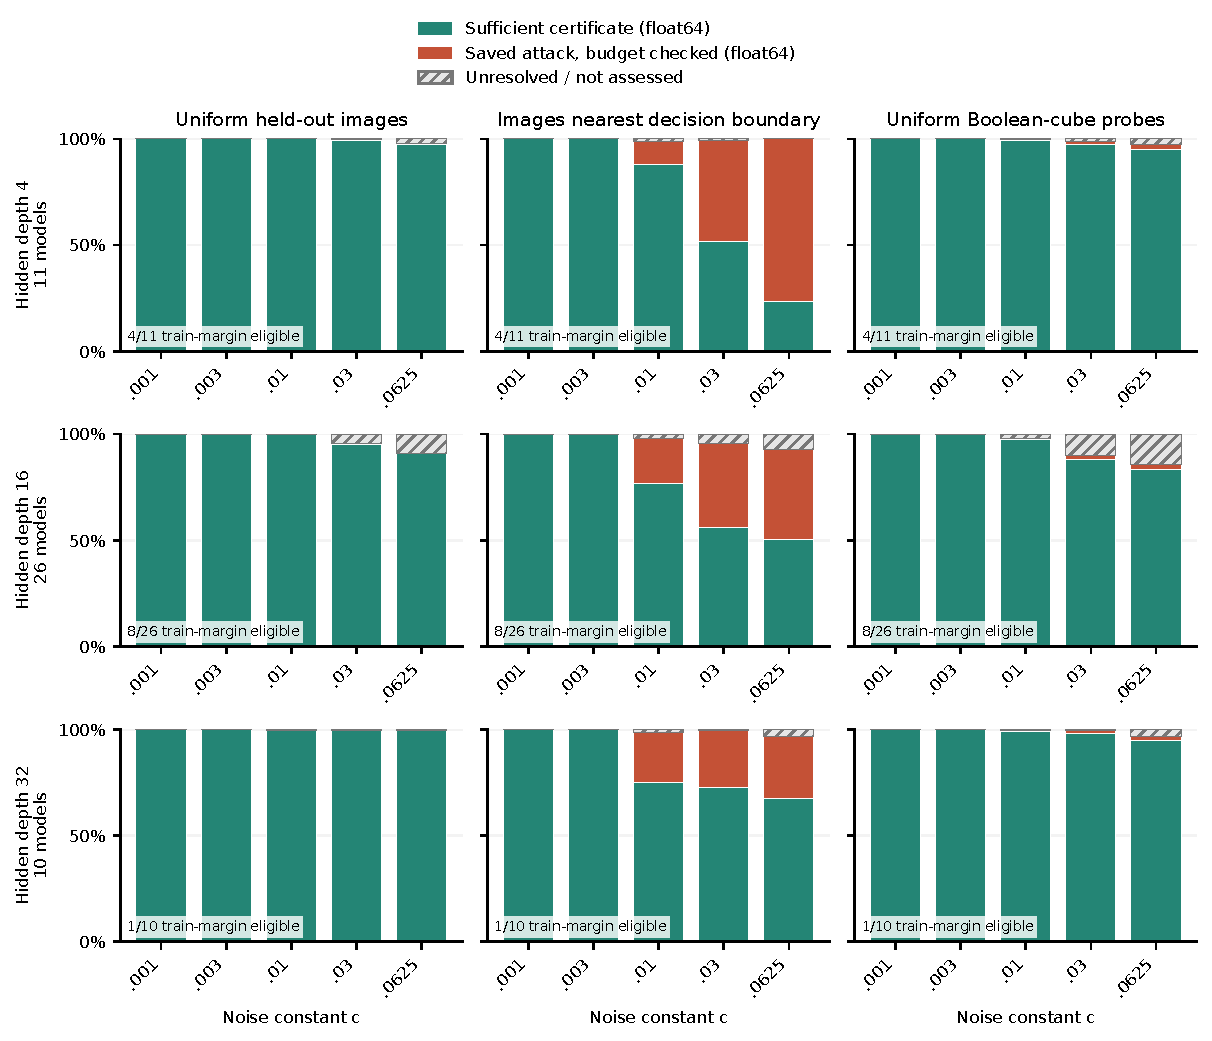
\includegraphics[width=.99\textwidth]{figures/certificate-coverage.pdf}
\caption{Fixed-subset audit of all depth-$4/16/32$ unconstrained tanh runs, including
failed training fits. Green denotes a sufficient finite-radius
certificate evaluated in float64; red denotes an explicit saved attack
that passes a float64 budget and score recheck; hatched gray denotes an
unresolved or unassessed point. Selected exact verifications are reported
separately. The same points and denominators are used at every radius.
Boundary images and uniform Boolean probes have different sampling
interpretations from uniformly selected test images.}
\label{fig:empirical-coverage}
\end{figure}

\paragraph{A same-model positive and negative result.}
The Boolean-input MNIST model \texttt{029} has hidden depth $16$, width
$128$, was trained by vanilla SGD, and has minimum training signed
output above $4.23$ and test accuracy $99.19\%$. Its raw output has a
global all-real-input certificate at $c=0.001$. At $c=0.01$, exact-budget
checks and outward interval arithmetic verify clipped-score violations
on both a held-out Boolean image and a uniform Boolean probe. The score
changes exceed $0.0845$ and $0.0855$, respectively. In both attacks every
disturbed hidden state remains in $[-1,1]$. Thus the calibration constant
matters even for a fitted classifier, and the larger-radius failures
are not caused by allowing hidden states outside the activation range.

The full-MNIST even-versus-odd model \texttt{104}, with hidden depth $4$
and width $256$, fits every training margin above $2.68$, reaches
$98.94\%$ test accuracy, and has an exact-rational global certificate
at $c=0.003$: its raw output changes by at most $0.03230<1/16$.
This certificate covers every real input, not merely the recorded
images. The statement concerns its trained parameterization; it does
not identify its training process with Bayesian inference.

The matched-task depth-$16$, width-$256$ model \texttt{105} illustrates
the limitation of a universal support claim. Exact integer/rational
verification puts all $60{,}000$ training signed margins above $4.48157$.
Certified clean-output intervals give $9{,}892$ correct predictions among
the $10{,}000$ test labels, confirming $98.92\%$ accuracy. Yet it has a rigorously
verified violation already at the primary constant
$c=0.001$. A synthesized 8-bit image with mean ink about $0.172$ and
$64.2\%$ black pixels has clean output approximately $-0.00163$ and
perturbed output $-0.15496$, giving clipped-score change above $0.1533$.
Every disturbed hidden state remains in $[-1,1]$. This is a constructed
off-distribution image, not a held-out natural image, and its encoding
into Boolean pixel bits is discussed separately. Thus fitting every
training margin does not by itself enforce the proposed global
condition.

A later, separately declared search addresses the objection that the
first witness starts near the decision boundary. On another synthetic
8-bit input, the same model has clean output in
$[0.53934,0.53935]$, above the training margin. A hidden-only disturbance
at $c=0.001$ lowers it to $[0.38661,0.38662]$, below $7/16$.
The scalar output disturbance is exactly zero, and every disturbed
hidden coordinate remains inside $[-1,1]$. Exact budget and outward
interval checks establish this for both rational pixel normalization
and the original float32 preprocessing. Thus the global failure also
affects a confident positive output and violates the training-level
implication~\eqref{eq:transport-training-level} of the optional two-margin
transport condition (Appendix~\ref{sec:two-margin-transport}); no true label is assigned to this
constructed image.

This failure is sharply separated from the observed image distribution.
A separately declared follow-up checked \emph{every} official held-out
image for selected models. For model \texttt{105}, all $10{,}000$ images
receive a sufficient pointwise certificate at both $c=0.001$ and
$c=0.003$. At the latter constant, $9{,}960$ pass by combining the global
raw-output bound with clipping, and the remaining $40$ pass using local
finite-radius bounds. Both original depth-$32$ MNIST SGD seeds similarly
certify all $1{,}984$ test images at both constants, despite their failed
training-margin fits. These initial whole-pool sweeps evaluate sufficient
inequalities in float64 on a finite held-out set; they do not cover every
natural image or the whole input cube.
Across all six prescribed follow-up models
(\texttt{005}, \texttt{008}, \texttt{009}, \texttt{029}, \texttt{105}, and
\texttt{107}), all $27{,}936$ held-out input/model pairs are certified
at both constants. Eleven initially unresolved points for model
\texttt{107} at $c=0.003$ were subsequently certified by stronger
finite-radius enclosures; that refinement history is retained.

Model \texttt{105} subsequently receives an exact upgrade at the primary
constant $c=0.001$: exact integer/rational arithmetic and outward
interval bounds certify every one of its $10{,}000$ official test inputs,
using their original float32-normalized values. A global bound covers
$9{,}988$ inputs and local bounds cover the remaining $12$, with maximum
certified clipped-score change below $0.017653<1/16$.
This quantifies over every allowed simultaneous disturbance at each of
those inputs. It does not certify unknown images or the population
distribution. The result at $c=0.003$ and the other models' whole-pool
results retain their float64 qualification.
The same exact method also verifies the training-margin statement above
and clipped-score stability at all $60{,}000$ training inputs at
$c=0.001$. Thus this model has verified likelihood eligibility and
verified stability on both official data sets while still failing the
global input-domain condition.

\paragraph{An explicit spectral-norm intervention.}
Four further vanilla-SGD runs project every hidden-to-hidden matrix
to operator norm at most $0.99$ after each epoch, including after the
final update. The first layer and readout are untouched. Each has a
matched unconstrained run with the same initialization, minibatch order,
data, number of gradient steps, and learning-rate schedule. The
nonexpansive certificate then guarantees score stability up to
$c=1/16$ when the saved internal norms are verified below one.
This is an intervention in training, rather than evidence that ordinary
SGD spontaneously enforces the condition. Its accuracy and training
margin cost must be assessed alongside the guaranteed stability.
The matched MNIST test accuracies change from $98.94\%$ to $98.95\%$
at depth $4$, and from $98.92\%$ to $98.87\%$ at depth $16$.
Fashion test accuracy decreases by $0.05$ and $0.65$ percentage points,
respectively. All four projected runs retain training errors and hence
fail the hard training-margin likelihood. They demonstrate useful
classification under an enforced support restriction, not fitted
examples under that likelihood.
The separately declared continuation for $240$ additional epochs of the depth-$16$
full-MNIST projected run still has $154$ training errors, compared with
$169$ initially, and test accuracy $98.83\%$. Thus the fixed longer
optimization budget does not resolve the training-likelihood failure.
All five projected parameterizations nevertheless have exact-rational
global certificates at $c=1/16$, including the continued model, whose
uniform raw-output variation bound is below $0.058087$.

\paragraph{A polynomial-depth calibration variant.}
After observing the fixed-radius failures, we also screened the
explicitly exploratory choice $c_H=0.001/H$. This weakens the radius by
one additional power of depth; a theorem polynomial in $c+c^{-1}$
continues to have polynomial depth dependence under this substitution.
For the same model \texttt{105}, exact-rational operator bounds certify
global raw-output variation at most $0.023658$ at $c_H=1/16000$, so
it passes this weaker condition on every real input. This does not
undo its failure at the original fixed constant. The larger-depth
cohort tests this variant further, without inferring an asymptotic
law from finitely many trained networks.
The fitted depth-$32$ continuation \texttt{301} yields the same
distinction: an interval-verified primary-radius violation coexists
with an exact global raw-variation bound below $0.017821$ at
$c_H=1/32000$. Its minimum training margin is $2.41066$ and test
accuracy is $99.244\%$; the other prescribed continuation still has
three training errors.

\IfFileExists{figures/projected-sgd-comparison.pdf}{
\begin{figure}[t]
\centering
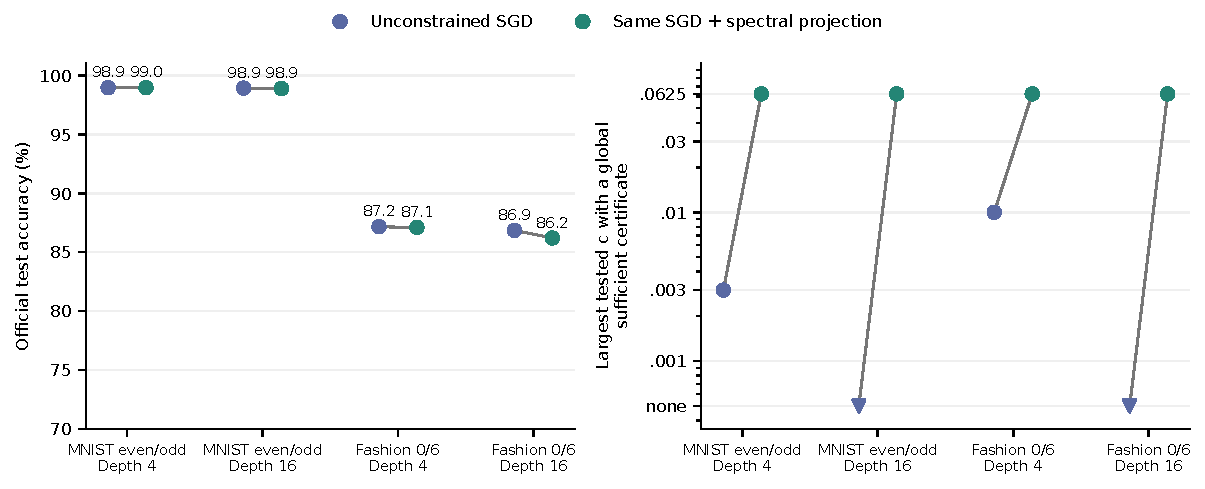
\includegraphics[width=.99\textwidth]{figures/projected-sgd-comparison.pdf}
\caption{Matched vanilla-SGD comparison with and without a spectral
projection after each epoch. The right panel gives the largest tested
radius constant with a global sufficient certificate, a lower bound
on stability rather than an estimate of the largest valid radius.
Training-margin eligibility is reported separately from accuracy.}
\label{fig:projected-comparison}
\end{figure}}{}

\paragraph{Reduced-precision diagnostic.}
We additionally round hidden activations to IEEE float16 or bfloat16,
leaving weights fixed, on the official test set. Hidden-only rounding
and hidden-plus-output rounding are separate modes. The realized joint
noise norm is recorded and compared with each calibrated radius. This
is one deterministic perturbation map, not a test of every allowed
perturbation and not a worst-case certificate. In particular, successful
rounding can occur even when its realized noise lies outside the
certified ball.
The smallest calibrated ball should not be equated with
ordinary low-precision arithmetic: the realized rounding budgets can
exceed it even when the classifier's clipped score barely changes.
The complete diagnostic reports both the score changes and the actual
noise-budget coverage.

\IfFileExists{experiment/quantization-results-table.tex}{\begin{table}[t]
\centering\small
\begin{tabular}{llrrrr}
\toprule
Format & Rounded values & Sign flips & Score changes $>1/16$ & $c=.001$ & $c=.0625$ \\
\midrule
float16 & Hidden & 1 & 0 & 0.00\% & 87.52\% \\
float16 & Hidden and output & 1 & 0 & 0.00\% & 32.28\% \\
bfloat16 & Hidden & 19 & 54 & 0.00\% & 1.22\% \\
bfloat16 & Hidden and output & 19 & 53 & 0.00\% & 0.05\% \\
\bottomrule
\end{tabular}
\caption{Deterministic activation-rounding diagnostic on 175,520 held-out input/model pairs across 60 tanh image models. The last two columns give the fraction whose realized joint noise lies inside the corresponding calibrated ball. The clipped score has cap $1/2$. Failures to fit the training likelihood are retained; no adversarial or distribution-wide claim follows from this fixed rounding map.}
\label{tab:quantization}
\end{table}
}{}

\paragraph{Exhaustive Boolean audit.}
Six additional networks use the exact domain $\{-1,1\}^9$, with target
either majority of the nine bits or majority of the three majorities
on disjoint groups of three. A fixed permutation selects $400$ training
and $112$ held-out inputs. Width is $64$, hidden depths are $4$, $16$,
and $64$, and every model receives the same prescribed $500$-epoch SGD
schedule. These models are reported separately from the image cohort.
The audit enumerates all $512$ inputs at the original five radius
constants and at $c_H=0.001/H$. Thus successful coverage concerns the
entire Boolean target domain, even when a sufficient bound uniform over
all real inputs is inconclusive. Domain coverage is exhaustive, but
the arithmetic is still float64 unless separately verified exactly.
All six runs fit the training margin empirically. The initial exhaustive
audit certifies all vertices at $c=0.001$ for five models, and $511$ of
$512$ for the remaining depth-$64$ recursive-majority model; all six
pass on every vertex at $c_H$. A separately recorded stronger bound
resolves the last vertex, enclosing its noisy raw output in
$[-2.45149,-2.36141]$ and hence giving zero clipped-score change.
Thus all six ultimately pass on the entire Boolean domain at the
primary constant. These finite examples test the support condition, not an
empirical sample-complexity law.

The predeclared first exact verification selected depth-$4$ majority
model \texttt{500} at $c=0.03$. Exact interval arithmetic verifies all
$400$ training signed margins above $1/2$ and all $512$ clean absolute
outputs above $4.72037$. Combined with an exact uniform raw-output
variation bound below $0.162903$, this proves that every clipped score
is constant throughout the allowed noise ball on the entire Boolean
domain. The raw variation bound exceeds $1/16$, so this certificate
uses clipping rather than merely a small raw-output bound; it does not
show that the network violates the raw-output stability condition.

A deeper exact positive is model \texttt{504}, the depth-$64$ majority
network. All $400$ training margins are interval-verified, and the
network correctly labels $511$ of the $512$ Boolean vertices. At the
primary constant $c=0.001$, an exact finite partition and reachable-tube
calculation proves zero clipped-score change on every vertex for every
allowed simultaneous perturbation. The scalar global raw-output bound
is approximately $13.4145$ and is insufficient on its own. Thus this
is a fitted deep SGD example satisfying the actual finite-domain
support condition, certified using the states reached by its inputs.
The depth-$64$ recursive-majority model \texttt{505} also receives an
exact all-domain certificate at $c=0.001$, combining $511$ reachable-tube
cases with an exact covariance calculation for the remaining vertex.
Every training margin is interval-verified above $7.47388$; it correctly
labels $504$ of the $512$ vertices. Both deep examples thus satisfy the
support condition without requiring perfect generalization.

\IfFileExists{experiment/boolean-results-table.tex}{\begin{table}[t]
\centering\small
\begin{tabular}{lrrrrrr}
\toprule
Target & $H$ & Min. margin & Test acc. & $c=.001$ & $c=.001/H$ & All-input $c_*$ \\
\midrule
Majority9 & 4 & 4.99 & 100.00\% & 512/512 & 512/512 & 0.0625 \\
Majority9 & 16 & 6.94 & 100.00\% & 512/512 & 512/512 & 0.0625 \\
Recursive majority & 4 & 4.04 & 100.00\% & 512/512 & 512/512 & 0.0625 \\
Recursive majority & 16 & 6.56 & 96.43\% & 512/512 & 512/512 & 0.03 \\
Majority9 & 64 & 7.61 & 99.11\% & 512/512 & 512/512 & 0.001 \\
Recursive majority & 64 & 7.47 & 92.86\% & 512/512 & 512/512 & 0.001 \\
\bottomrule
\end{tabular}
\caption{Exact finite Boolean domains, with float64 evaluation of sufficient finite-radius inequalities. Certified counts cover all $512$ inputs; $c_*$ is the largest original-grid constant for which every input passes, a lower bound on the valid radius rather than an estimate of its maximum. The minimum margin is over the $400$ training inputs. One initially unresolved vertex at $c=.001$ receives a separately recorded stronger certificate. A failed sufficient certificate remains unresolved; it is not a counterexample.}
\label{tab:boolean-fullcube}
\end{table}
}{}

The experiment directory preserves protocols, raw weights, dataset
hashes, per-example outputs, failed fits, all saved attack witnesses,
certificate records, and plotting code. Exact proofs, pointwise
numerical evidence, and empirical training outcomes have distinct
qualifications throughout.
}{}
\IfFileExists{certificates/report-fragment.tex}{% Included after the empirical overview. These are selected independently
% verified examples, not additional population-level empirical tables.
\section{Independent finite-radius verification of trained networks}
\label{sec:verified-trained-networks}
The aggregate empirical audits above use numerical sufficient inequalities and numerical attacks.  This section separates out selected positive and negative examples checked by exact rational arithmetic and outward interval evaluation.  A certificate for all real inputs is distinguished from an exhaustive certificate on a specified finite Boolean domain.  Both quantify over every allowed disturbance.  A pointwise certificate covers every disturbance at one specified input, while a negative witness is one verified input--disturbance pair.  These scopes are kept distinct.

\paragraph{Global certificates for raw trained models.}
The global restriction is satisfied by some ordinary, unconstrained trained networks.  A width-256, depth-4 tanh network trained by minibatch SGD on all 60,000 MNIST images for even-versus-odd classification has test accuracy $98.94\%$, no training errors, and minimum signed training output exceeding $2.6876$.  Its raw saved weights satisfy the global condition at $c=.003$: for every real input and every allowed simultaneous disturbance, the raw output changes by at most $0.032296<1/16$.  This global bound was verified using exact rational operator-norm certificates and a rational final gain comparison, rather than relying on a floating-point spectral estimate.

There are also eligible depth-16, width-128 examples at $c=.001$: the selected SGD models for continuous and thresholded-Boolean MNIST 3-versus-8 inputs have minimum training margins exceeding $.6918$ and $4.236$, respectively, test accuracy $99.29\%$ and $99.19\%$, and rigorously verified global raw-change bounds $.060795$ and $.062230$.  These use raw trained weights, without output rescaling.  Their global certificates apply to every real input, so imply either clipped-score convention.  The radius constant matters: for the latter Boolean model we independently verified violations at $c=.01$ on both a held-out image and a Boolean cube probe, with clipped-score changes exceeding $.08450$ and $.08553$, respectively.  The successful small-radius certificate and larger-radius failure are compatible.

\paragraph{An exploratory inverse-depth calibration.}
A later, separate calibration sets $c_H=.001/H$.  For the depth-16 full-MNIST model \texttt{105}, which has a verified global failure at the original $c=.001$, exact rational spectral bounds prove global raw-output variation at most $.02365730<1/16$ at $c_H=1/16000$.  Thus this same trained parameterization passes a weaker, explicitly depth-dependent support condition.  This is not a revision of the original protocol or evidence that a fixed $c$ works uniformly in depth.  Since the theoretical bound has polynomial dependence on $c+c^{-1}$, such a polynomial depth calibration preserves a polynomial formal sample bound.  The training-eligible depth-$32$ continuation \texttt{301} also has an exact global raw-change bound $.01782087$ at $c_H=1/32000$, despite its verified failure at fixed $c=.001$.

\paragraph{Projected SGD at a larger fixed radius.}
All four predeclared projected-SGD models (depths $4$ and $16$, width $256$, on full MNIST parity and Fashion-MNIST shirt-versus-T-shirt) have exact rational certificates that every internal matrix has operator norm below one.  Their global raw-output change bounds at $c=1/16$ are respectively $.061573$, $.058087$, $.061573$, and $.058087$, all below $1/16$.  The corresponding test accuracies are $98.95\%$, $98.87\%$, $87.10\%$, and $86.20\%$.  None attains every training margin above $1/2$: this is evidence that the support condition can coexist with useful trained prediction, not an example satisfying the paper's exact interpolation likelihood.
The separately declared longer-training continuation \texttt{600} retains an exact global bound $.058087$ at the same radius, but still has $154$ training errors after $240$ additional epochs, with $98.83\%$ test accuracy.  Thus all five projected parameterizations have verified global stability, and none is presented as satisfying the exact training-likelihood event.

\paragraph{Exhaustive Boolean-domain certificates.}
A separate, predeclared cohort trains width-$64$ tanh networks on $400$ of the $512$ vertices of $\{-1,1\}^9$, with the remaining $112$ vertices held out.  For the protocol-selected depth-$4$ majority network \texttt{500}, exact arithmetic and outward intervals certify the clipped-score condition on \emph{every} Boolean input at $c=.03$.  All $400$ training margins are independently interval-verified above $1/2$, and the network correctly predicts all $512$ labels.  The global raw-change bound is $.162903>1/16$, whereas every clean absolute output exceeds $4.72037$.  Consequently the clipped score is exactly constant under every permitted disturbance at every vertex.  A separate auditor replayed the saved matrix factors, all $512$ interval trajectories, and all $400$ training inequalities.

A subsequent, separately recorded check gives the same exhaustive conclusion for the depth-$16$ majority network \texttt{501} at the largest primary radius $c=1/16$.  Its raw-change bound is $3.474718$, while every clean absolute output exceeds $5.12034$; all $512$ labels and every training margin are correct.  These finite-domain certificates use the elementary implication
\[
 |z(x)|\ge m,\qquad |z^\eta(x)-z(x)|\le B\le m-\tfrac12
 \quad\Longrightarrow\quad
 \operatorname{clip}_{1/2}(z^\eta(x))=\operatorname{clip}_{1/2}(z(x)).
\]
They therefore certify the actual clipped-score condition even when the stronger raw-output-change condition is not certified.  Their scope is the entire finite Boolean domain, not all real inputs.

\paragraph{A depth-$64$ example requiring reachable-state bounds.}
The first depth-$64$ majority network, \texttt{504}, also satisfies the condition on \emph{all} $512$ Boolean vertices at the primary $c=.001$.  Every one of the $400$ training margins is interval-verified above $7.61170$, and every clean absolute output on the full cube exceeds $5.64786$.  Thus this network also satisfies the original all-input clean-margin restriction, not only the newer clipped-score restriction.  Exact interval label comparisons give $511/512$ correct predictions on the full cube, including $111/112$ held-out predictions; the remaining vertex is a confidently wrong prediction, not an omitted or ambiguous case.  Its global raw-change bound, $13.414533$, cannot establish this conclusion, even with output clipping.  Instead, $52$ finite groups of vertices share rigorously bounded reachable-state tubes.  Each group's disturbed outputs remain beyond the corresponding clipping threshold, with the smallest verified surplus exceeding $1.40770$.  Thus the clipped score is exactly invariant for every allowed disturbance at every vertex.  This is an exhaustive finite-domain certificate for an ordinary SGD-trained depth-$64$ network, rather than a sampled-input audit or a claim about every real input.

For completeness, sharing a tube across finitely many inputs does not alter the underlying proof.  At each layer and coordinate, replace the clean preactivation's distance from zero by the minimum of that distance over all vertices in the group.  A common prefix-energy bound then encloses every group's noisy trajectory, so the same derivative and matrix-norm bounds apply to each vertex.  The grouping only reduces computation.  Every input is still checked, and any unresolved input would prevent a full-domain conclusion.  The certificate uses exact integer matrix arithmetic, outward interval $\tanh$, saved norm-factor proposals, and explicit source hashes; it is not a Lean proof.  A separate auditor regenerated all $512$ clean interval trajectories, checked all $52$ groups and $3{,}216$ saved matrix bounds, and replayed every training inequality.  The three worst groups were additionally checked with the original pure-integer matrix-norm verifier.

\paragraph{A depth-$64$ nonlinear target.}
The corresponding recursive-majority network \texttt{505}, trained on majority of three disjoint three-bit majorities, also satisfies the clipped-score condition on the entire $512$-vertex cube at $c=.001$.  Every one of its $400$ training margins is interval-verified above $7.47388$, and every clean absolute output exceeds $2.40649$, so the original all-input clean-margin condition holds as well.  Its full-domain accuracy is $504/512$; the held-out accuracy is $104/112$.  All eight errors remain in the verified domain.

For this network, the shared reachable-tube proof establishes $511$ of the $512$ cases.  The remaining vertex, index $325$, is explicitly retained as unresolved in that component certificate.  A separate finite-radius proof propagates the exact clean-response covariance and bounds the nonlinear Taylor remainder in state norm.  It encloses the noisy output at this same vertex in $[-2.586691,-2.226290]$, proving that its clipped score is also invariant.  The composite certificate records the union of these two proofs, with model, radius, source, and component hashes; the input domain never changes.  The exceptional-vertex proof was independently replayed, including all $126$ exact matrix-norm bounds.  A further independent replay regenerated all $512$ clean trajectories, all $122$ groups and $7{,}585$ local matrix bounds, and every training margin, then checked the composite coverage.  The state-covariance inequality used for this refinement is given below.

\subsection{The global condition can fail on valid finite-grid inputs}
\label{sec:finite-grid-counterexamples}
A universal prior-support restriction and a statement about typical data are different claims.  The distinction persists after clipping at the training margin, even for a network that fits all training examples with substantial margin.  Our strongest example is an ordinary minibatch-SGD tanh network of hidden depth 16 and width 256, trained on all 60,000 MNIST images for even-versus-odd classification.  It has $98.92\%$ empirical test accuracy, and a separate exact computation verifies every signed training output above $4.4815762$.  The finite-radius counterexample below is independently verified.  The saved weights are used without rescaling.

The left image in Figure~\ref{fig:finite-grid-counterexamples} is a valid $28\times28$ eight-bit grayscale input.  At the smallest tested radius constant $c=10^{-3}$, its clean and disturbed real outputs are enclosed around
\[
 -0.00162845134\longmapsto-0.15496440197.
\]
The resulting score change exceeds $0.15333>1/16$ after clipping at either $1/2$ or $1$.  The image has a black two-pixel border, mean ink $0.17200$, and $64.2\%$ black pixels.  It is a synthetic off-data image, not an image to which we assign a natural digit label.  Its pixel $p_j$ is interpreted as the exact rational input $x_j=2p_j/255-1$; we also independently checked the same witness under the original float32 pixel preprocessing used for training.

The disturbance budget was checked using exact integer-rational arithmetic, and the two network evaluations used 100-decimal outward interval arithmetic with the saved dyadic weights.  In particular,
\[
 (1+H E_v)\left(N^{-1}\sum_{s=1}^{H}\|\eta_s\|_2^2+\xi^2\right)
 <10^{-6}.
\]
The intervals verify that every perturbed hidden coordinate remains in $[-1,1]$: their absolute values are all below $0.061110$.  Thus requiring disturbances to leave activations within their original range does not remove this counterexample.  Its scalar output disturbance has absolute value below $7.3\times10^{-10}$.  Removing it decreases the noise budget and changes either clipped score by at most that amount, so hidden disturbances alone still give a violation.  These are finite-radius witnesses, rather than conclusions drawn only from a large Jacobian or from an unverified optimization output.  They trust the interval-arithmetic implementation and are not Lean formalizations.

The right image provides a second example in a depth-32, width-128 SGD model for MNIST 3 versus 8, with test accuracy $99.09\%$.  Its output changes from $-0.0034068096$ to $-0.3168576499$ at the same $c=10^{-3}$, a clipped-score change greater than $0.31345$.  All perturbed hidden coordinates have absolute value below $0.128211$.  This second model has three training errors, so it is evidence about the naturalness of a support restriction rather than an additional example in the exact training-likelihood event.  A related near-gray eight-bit witness for this model has score change greater than $0.30799$.  The low-ink examples exclude an explanation specific to a uniformly gray background, while remaining clearly off-data.

Each exploratory search had a fixed budget declared before that search.  For the low-ink examples we solved an ink-minimizing linear program, subject to zero first preactivations and a black border, generated 4,096 stochastic roundings to the pixel grid using a fixed seed, and attacked the 16 candidates with smallest absolute clean output.  We then verified selected witnesses independently.  This protocol proves existence, not the prevalence of instability under the data distribution.  In separate probes preserving empirical one-pixel foreground probabilities and on interpolations of opposite-class test images, some violations were verified at $c=10^{-2}$; failure to find violations at smaller radii was not treated as a certificate.

\begin{figure}[t]
\centering
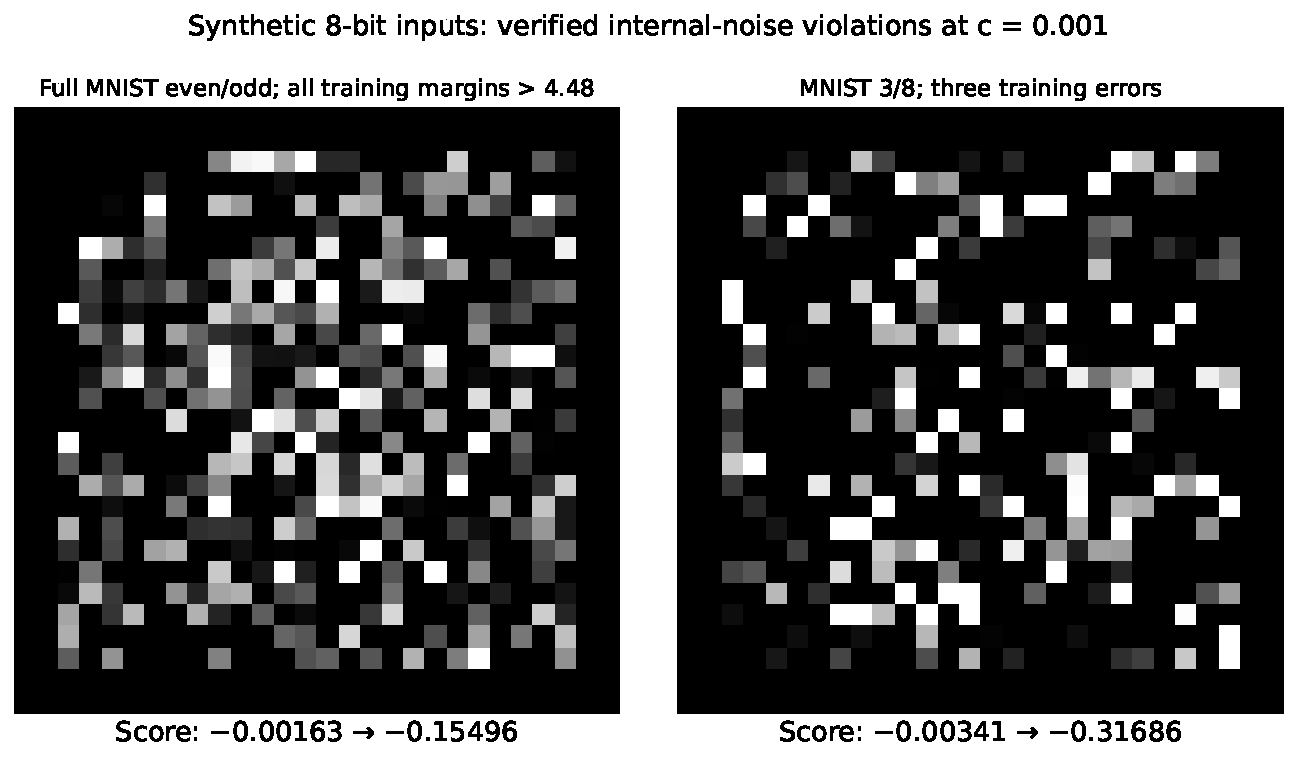
\includegraphics[width=.98\linewidth]{certificates/finite-grid-counterexamples.pdf}
\caption{Synthetic, valid eight-bit inputs violating the global clipped-score condition at $c=.001$.  Both have a fixed black border and low total ink.  The left network was trained on the full MNIST even-versus-odd task and has exactly verified training margins above $4.4815762$; the right network was trained on digits 3 and 8.  The images themselves are unchanged by the internal disturbances.  These are off-data counterexamples, not mislabeled examples from a test set.}
\label{fig:finite-grid-counterexamples}
\end{figure}

\paragraph{A precise Boolean interpretation.}
The finite-grid issue is not inherently a continuous-input phenomenon.  Write each pixel in bits $p_j=\sum_{b=0}^7 2^b q_{jb}$, with $s_{jb}=2q_{jb}-1\in\{-1,1\}$.  Since $\sum_b2^b=255$,
\[
 \frac{2p_j}{255}-1=\sum_{b=0}^7\frac{2^b}{255}s_{jb}.
\]
Replacing row $j$ of the first-layer matrix by eight rows $(2^b/255)W_{0,j}$ gives a network on $8\cdot784=6272$ Boolean inputs with exactly the same outputs, hidden trajectories, readout energy, and internal-noise budgets.  Its depth and width are unchanged.  Thus every rational-pixel witness is also an exact Boolean-input witness for this linearly decoded network.  With the usual dimension-weighted first-layer Frobenius energy, the non-bias weight contribution grows only by
\[
 8\sum_{b=0}^7(2^b/255)^2
 =\frac{8(4^8-1)}{3\cdot255^2}<2.69.
\]
The first-layer bias is unchanged but its dimension weight grows eightfold.  Consequently total first-layer energy, including the bias, increases by at most a factor of eight.
This equivalence uses exact rational pixel normalization.  The software used to train and evaluate the original model normalizes pixels in float32; the original-preprocessing witnesses were checked separately, and the held-out empirical audits use precisely those float32-normalized inputs.  We do not identify the two normalization maps as exact equalities.

\paragraph{An optional margin-band score.}
As a separate, post-protocol comparison, consider
$U(z)=\operatorname{sign}(z)\min\{1/4,(|z|-1/4)_+\}$, which ignores changes entirely inside the already-failing test-margin band.  The original depth-32 low-ink witness still violates its $1/16$ condition, with $U$-score change greater than $0.0668576$; its near-gray witness does not.  For the fitted full-MNIST depth-16 model, the zero-centered witness lies entirely within the ignored band.  We therefore declared a new, explicitly variant-specific exploratory protocol: move the continuous low-ink input toward clean output $3/8$, generate 4,096 pixel-grid roundings, retain the 16 closest to $3/8$, and apply the same internal-noise attack budget.  The independently verified witness has
\[
 z=0.3628586342\longmapsto0.5158098496,
 \qquad |\Delta U|>0.1371413>1/16
\]
at $c=.001$.  All disturbed hidden coordinates have absolute value below $0.089882$.  Here too the scalar output disturbance is below $7.3\times10^{-10}$, so the same $1$-Lipschitz argument gives a hidden-disturbance-only violation.  This secondary result shows that the weaker score can move the fragile input region without eliminating the global obstruction; it does not change the primary clipped-score protocol.

The predeclared longer-training check also supplies a depth-$32$ example.  Of the two fixed continuations, model \texttt{301} fits all $11{,}982$ training examples with minimum signed output above $2.4106$ and achieves $99.24\%$ held-out accuracy.  A valid low-ink, black-border 8-bit image has interval-verified output change $-.00895437\mapsto+.30415992$ at $c=.001$, hence clipped-score change exceeding $.31311$.  Every noisy hidden state remains in $[-1,1]$.  The other continuation retains three training errors; both outcomes and both prescribed searches are retained.  Training metrics in this paragraph are ordinary float64 evaluations, whereas the displayed counterexample has an exact rational noise-budget check and outward interval forward evaluation.

A still weaker, exploratory implication-only condition asks that, for both labels $y$, $yz\ge1/2$ imply $yz^\eta\ge7/16$, and $yz\le1/4$ imply $yz^\eta\le5/16$.  Negating the already saved perturbation for model \texttt{301}, without any new optimization or input selection, yields the interval-verified output $-.32205298$ from the same clean value $-.00895437$.  With $y=-1$, the second implication fails.  Its margin-band score also changes by more than $.07205>1/16$.  The exact noise budget is unchanged by negation and every disturbed hidden state remains in $[-1,1]$.  This auxiliary check concerns later proposed variants; it does not change the primary score convention or empirical protocol.

\paragraph{Failure starting from a confident output.}
A further, separately declared finite-budget check targets clean output $.55$ in the fitted full-MNIST model \texttt{105}.  The resulting valid eight-bit, low-ink input has independently replayed interval enclosures around
\[
 z=0.539345460246\longmapsto z^\eta=0.386611305539
 \qquad(c=.001).
\]
Here the scalar output disturbance is exactly zero.  The exact rational hidden-noise budget passes, and every disturbed hidden coordinate has absolute value below $.101215$.  Thus the first implication above fails for $y=+1$: a clean signed output above $1/2$ falls below $7/16$.  Both the clipped score and the optional margin-band score change by more than $.113388>1/16$.  The same saved disturbance was independently verified under the original float32 pixel preprocessing.  The input is synthetic and has no assigned digit label; the positive clean output establishes the implication's premise.  This check refutes an explanation of the observed instability based solely on clean outputs near zero.  It does not show that this image model satisfies the original all-input clean-margin restriction, which its other near-zero inputs already violate.

\subsection{Exact stability on the complete held-out image set}
For the same fitted full-MNIST depth-$16$, width-$256$ model \texttt{105}, we can verify the primary clipped-score condition on \emph{every one of the $10{,}000$ official held-out images} at $c=.001$.  This includes incorrectly classified images; the certificate concerns stability, not correctness.  It uses the exact float32-normalized inputs of the training and evaluation pipeline and quantifies over every allowed simultaneous hidden/output disturbance at each such input.

A separate exact pass also verifies \emph{all $60{,}000$ signed training margins}, with a minimum certified lower bound exceeding $4.4815762>1/2$.  Every training input satisfies the clipped-score condition at $c=.001$ as well.  Thus, for this particular image model, training-likelihood eligibility is verified by exact arithmetic rather than inferred only from the float64 training metrics.  Exact sign comparisons against every archived test label also confirm $9{,}892$ correct and $108$ incorrect predictions, with no ambiguous cases, reproducing the $98.92\%$ test accuracy.

A guarded integer computation with rigorously enclosed activation-table and quantization errors gives a clean-output interval at every image, with uniform scalar error below $.007149522$.  Combining these intervals with an exact global disturbance bound certifies $9{,}988$ images.  The remaining $12$ inputs are explicitly retained as unresolved in that component record.  Separate $160$-bit interval clean trajectories, exact reachable-tube matrix bounds, and signed Taylor-remainder certificates prove those same $12$ cases.  The largest certified clipped-score change over the complete set is below $.01765217<1/16$.  A hash-checked composite record verifies that the two components cover precisely indices $0,\ldots,9{,}999$, with the same model, input archive, and radius.

The integer clean-output computations were independently repeated, reproducing all $10{,}000$ test and $60{,}000$ training rational row records exactly.  A separate replay also reproduced every exact rational row of all $12$ local certificates, and the complete-set composition was independently checked.  The worst local case received an additional replay of every matrix bound using the original pure-Python-integer verifier.  These are exact integer/rational and outward-interval sufficient proofs, not ordinary float64 sufficient tests and not Lean formalizations.  The analogous larger-radius $c=.003$ audit remains numerical.

This finite-set result coexists with the independently verified synthetic-input failures at the same $c=.001$, including the confident-input witness above.  It therefore establishes a precise distinction between stability on every image in the official test set and stability over every possible image.  It does not prove uniform stability on a neighborhood of those images or a distributional coverage guarantee.

\subsection{A limited test of a smooth-image trusted region}
\label{sec:smooth-trusted-region}
The preceding low-ink images are visibly atypical.  We therefore tested a separate, simple image restriction based on anisotropic total variation,
\[
 \operatorname{TV}(p)=\sum_{(i,j)\in\mathcal E}|p_i-p_j|,
 \qquad p\in[0,1]^{784},
\]
where $\mathcal E$ consists of horizontal and vertical nearest-neighbor edges.  The 10,000 official MNIST test images have median TV $102.55$, 99th percentile $143.74$, and maximum $180.41$.  These image statistics do not themselves establish that an input is natural.

For the fitted depth-16 full-MNIST model \texttt{105}, we minimized TV subject to zero first preactivations, a black two-pixel border, and mean ink at most $1/5$.  The resulting rounded eight-bit image remains a verified counterexample at $c=.001$, but its TV is $284.93$, above every test image.  This search therefore does \emph{not} refute a trusted region with TV at most $150$.

We can rigorously exclude this particular mechanism from that region.  An exact rational dual certificate gives
\[
 \operatorname{TV}(p)\ge284.87765209159
\]
for every image satisfying the stated border and ink constraints and exactly zero first preactivations.  More generally, the same certificate implies that an image in the border/ink region with TV at most $150$ has
\[
 \max_i |a_{1,i}|\ge0.1175517.
\]
These claims exclude zero and uniformly near-zero first states; they do not bound the later Jacobians or prove stability on the region.

A separately declared check gives the same qualitative conclusion for the fitted depth-$32$ model \texttt{301}.  Its exact rational dual certificate proves TV at least $287.04761391129$ for a zero first state under the same border and ink constraints.  TV at most $150$ instead forces maximum absolute first preactivation at least $.26750111067$.  None of the $4{,}097$ prescribed nearest and stochastic pixel-grid roundings of the numerical minimizer entered the region.  These are additional exclusions of this particular construction, not a uniform output-stability certificate or evidence that every fragile input has high TV.

For completeness, the certificate does not assume that the numerical linear-program solver is correct.  In normalized coordinates $x=2p-1$, introduce $t_e\in[0,2]$ with $\pm(x_i-x_j)\le t_e$, so TV is one half of the linear objective $\sum_e t_e$.  Write the resulting problem as minimizing $c^Ty$ with equality constraints $Ay=b$, inequalities $By\le d$, and coordinate box $l\le y\le u$.  For arbitrary exact dyadic multipliers $\lambda$ and $\mu\le0$, put $q=c-A^T\lambda-B^T\mu$.  Then
\[
 c^Ty\ge \lambda^Tb+\mu^Td+
       \sum_j\min\{q_jl_j,q_ju_j\}.
\]
We evaluate this expression using integer-rational arithmetic against the actual stored first-layer weights.  It remains valid even when the proposed dual multipliers are inaccurate.  If the equality constraint is violated by a first-preactivation vector $a_1$, the right side decreases by at most $\|\lambda\|_1\|a_1\|_\infty$; dividing by two gives the stated near-zero exclusion.  The exact coefficients and bound are saved for replay.

A complementary, separately declared stress test interpolated 256 deterministic opposite-parity pairs of correctly classified held-out MNIST images, using endpoints with TV at most $140$, ink at most $.195$, and black two-pixel borders.  We bisected toward output $0$ and $3/8$, rounded to eight-bit pixels, and retained all 512 rounded candidates satisfying TV at most $150$, ink at most $.2$, and the same border condition.  We attacked the 32 candidates with largest clean internal-noise gain for each target.  All 64 selected inputs pass the numerical finite-radius sufficient tests at $c=.001$ and $.003$, for both scores.  These are float64 evaluations of rigorous real inequalities, not interval proofs.  The corresponding attacks found no violations; that observation is not used as a substitute for the sufficient tests.

At $c=.01$, all 64 selected inputs have numerical primary-score violations.  Independently verified examples have TV $88.93$ and $100.13$, and mean ink $.118$ and $.158$.  To test disturbances confined to valid activation states, we set one offending noise coordinate to zero in each selected witness and reverified the resulting trajectories: all hidden states remain in $[-1,1]$, while the primary score changes by more than $.1474$ and the optional margin-band score changes by more than $.1384$, respectively.  The exact pixel sums verify the region constraints.  Figure~\ref{fig:tv-boundary-counterexample} shows one such interpolation.  Therefore a TV/ink restriction excludes the zero-state counterexample mechanism and improves this stress test at the smaller radii, but does not ensure the larger-radius condition.  No conclusion of uniform stability on the trusted region follows from these finite samples.

\begin{figure}[t]
\centering
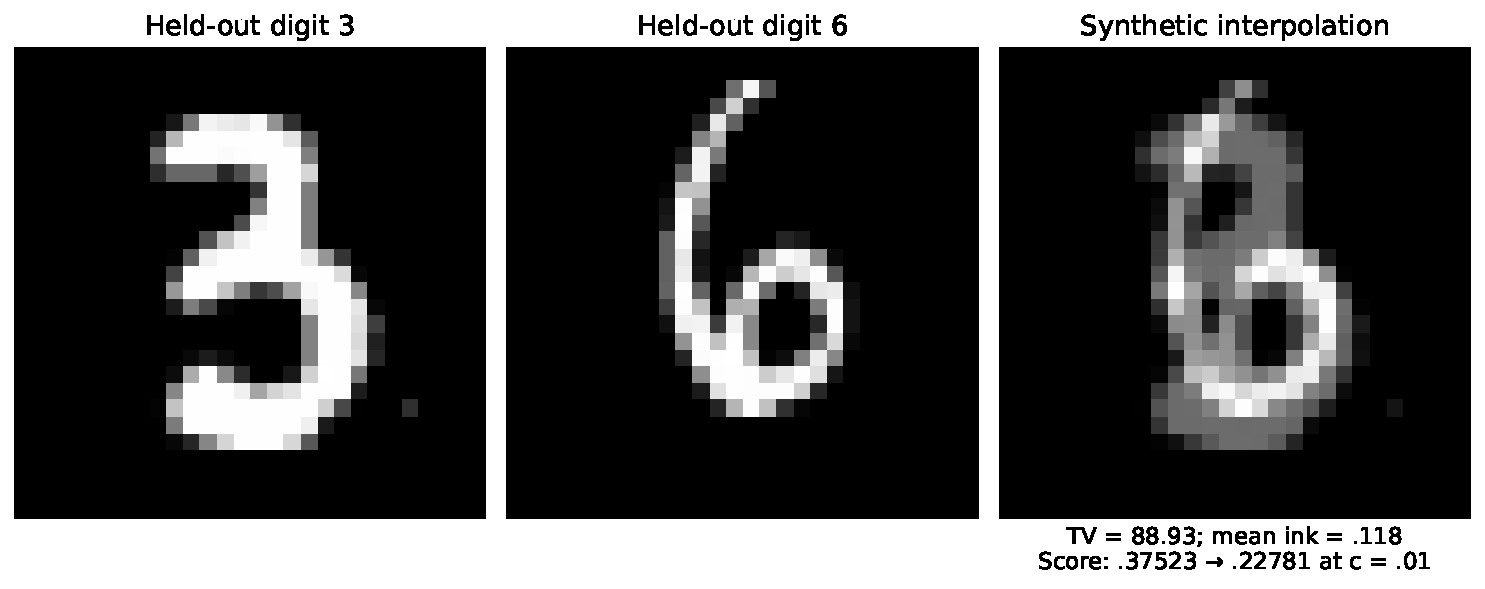
\includegraphics[width=.95\linewidth]{certificates/tv-boundary-counterexample.pdf}
\caption{An interpolation of opposite-parity held-out images, rounded to the eight-bit grid.  The interpolated image is synthetic and is not assigned a parity label.  At $c=.01$, a verified internal disturbance changes its clipped score by more than $.1474$, while every hidden state stays in $[-1,1]$.  Its TV and mean ink are within the stated smooth-image region.  This is a larger-radius example; the selected interpolation set passes numerical sufficient tests at $c=.001$ and $.003$.}
\label{fig:tv-boundary-counterexample}
\end{figure}

\section{Finite-radius certificates using reachable activation states}
\label{sec:reachable-tube}

A product of global operator norms ignores saturation. The following
certificate uses activation ranges reachable from one clean input under
\emph{all} disturbances in the prescribed ball. It applies at any radius;
small radii are not needed for its logical validity. The resulting bounds
can become conservative or vacuous at large radii.

Write the hidden network in column-vector notation as
$h_s=\tanh(a_s)$, $a_s=A_sh_{s-1}$, $1\le s\le H$, with a scalar readout
$z=v^\top h_H$. The input and its bias coordinate are fixed. Add
postactivation disturbances $\eta_s$ and output disturbance $\xi$, with
\[
 \sum_{s=1}^H\|\eta_s\|_2^2/N+\xi^2\le r^2.
\]
All clean activations, preactivations, and derivative matrices
$D_s=\operatorname{diag}(\operatorname{sech}^2a_s)$ below are fixed by this
input. Set $J_s=D_sA_s$ for $s\ge2$.

\paragraph{Forward enclosures.}
We construct a scalar $B_s$ and a nonnegative vector $C_s$ satisfying,
simultaneously for every allowed disturbance,
\[
 \|\Delta h_s\|_2\le B_s,\qquad |\Delta h_s|\le C_s.
\]
Initialize
$B_1=\sqrt N r$, $C_1=\sqrt N r\,\boldsymbol1$,
$q_1^{\rm lin}=q_1^{\rm tube}=1$, and $e_1=0$.
Given the preceding enclosures, set componentwise
\[
 b_{s,i}=\min\{\|(A_s)_{i,:}\|_2 B_{s-1},
                        (|A_s|C_{s-1})_i\}.
\]
Then the perturbed preactivation lies in
$[a_{s,i}-b_{s,i},a_{s,i}+b_{s,i}]$.
For the scalar remainder
\[
 R_a(u)=\tanh(a+u)-\tanh(a)-\operatorname{sech}^2(a)u,
\]
compute bounds $\rho^-_{s,i}\le R_{a_{s,i}}(u)\le\rho^+_{s,i}$ for
$|u|\le b_{s,i}$. Its exact extrema occur among the endpoints, $u=0$,
and $u=-2a_{s,i}$ when this point belongs to the interval: the derivative
vanishes exactly when $a+u=\pm a$. These extrema may be intersected with
any valid quadratic curvature bound. Put
$\rho_{s,i}=\max\{|\rho^-_{s,i}|,|\rho^+_{s,i}|\}$.

Choose upper bounds $\ell_s\ge\|J_s\|_{\rm op}$ and
\[
 L_s\ge\|U_sA_s\|_{\rm op},\qquad
 U_s=\operatorname{diag}\!\left(
  \operatorname{sech}^2((|a_{s,i}|-b_{s,i})_+)\right).
\]
Update
\begin{align*}
 q_s^{\rm lin}&=1+\ell_s^2q_{s-1}^{\rm lin},&
 e_s&=\ell_se_{s-1}+\|\rho_s\|_2,\\
 q_s^{\rm tube}&=1+L_s^2q_{s-1}^{\rm tube},&
 B_s&=\min\{\sqrt N r\sqrt{q_s^{\rm lin}}+e_s,
                    \sqrt N r\sqrt{q_s^{\rm tube}}\}.
\end{align*}
Finally set
\[
 C_{s,i}=\min\!\left\{B_s,\sqrt N r+
   \max_{u\in\{-b_{s,i},b_{s,i}\}}
          |\tanh(a_{s,i}+u)-h_{s,i}|\right\}.
\]
These intersections combine independent valid enclosures; they do not
assume that every disturbance can attain all their endpoints together.

\paragraph{Why the forward bounds hold.}
The exact perturbed recurrence is
$\Delta h_s=J_s\Delta h_{s-1}+\eta_s+R_s$, where $R_s$ lies in the
specified componentwise remainder interval. The sum of the clean linear
responses to all $\eta_j$ has norm at most
$\sqrt N r\sqrt{q_s^{\rm lin}}$, by Cauchy--Schwarz over the layerwise
noise norms and the products of the $\ell_j$. The propagated remainder
has norm at most $e_s$.
Independently, every mean-value derivative on the reachable interval has
coordinatewise absolute value bounded by $U_s$. Its operator norm is
therefore at most $\|U_sA_s\|_{\rm op}$: writing its diagonal derivative
as a diagonal contraction times $U_s$ proves this assertion.
Telescoping the nonlinear recurrence and using Cauchy--Schwarz now gives
$\sqrt N r\sqrt{q_s^{\rm tube}}$. The coordinate bound follows by
monotonicity of $\tanh$ and $|\eta_{s,i}|\le\sqrt N r$.
These arguments close the induction, including the use of the previously
intersected scalar and coordinate bounds to construct each new tube.

\paragraph{An output-specific interval.}
Define clean reverse adjoints
\[
 g_H=v,\qquad g_{s-1}=J_s^\top g_s,
 \qquad G=\sqrt{1+N\sum_{s=1}^H\|g_s\|_2^2}.
\]
Set $\rho_1^-=\rho_1^+=0$ and
\[
 E^- =\sum_{s,i}\min\{g_{s,i}\rho^-_{s,i},g_{s,i}\rho^+_{s,i}\},\qquad
 E^+ =\sum_{s,i}\max\{g_{s,i}\rho^-_{s,i},g_{s,i}\rho^+_{s,i}\}.
\]
Then every allowed disturbed output belongs to
\begin{equation}\label{eq:reachable-output-interval}
 [z-rG+E^-,\ z+rG+E^+].
\end{equation}
Indeed the exact output difference is
$\xi+\sum_sg_s^\top\eta_s+\sum_sg_s^\top R_s$.
The first two terms have absolute value at most $rG$; the last terms lie
between $E^-$ and $E^+$. One may further intersect this interval with
\[
 [z-T,z+T],\qquad
 T=r+\min\{\|v\|_2B_H,\ |v|^\top C_H\}.
\]
In particular these are finite-radius statements, not merely clean
Jacobian estimates.

For the clipped score $\psi_a(z)=\max\{-a,\min\{a,z\}\}$ and any verified
output interval $[l,u]$, the sufficient stability test is
\[
 \max\{|\psi_a(l)-\psi_a(z)|,|\psi_a(u)-\psi_a(z)|\}\le1/16.
\]
The main empirical convention uses $a=1/2$, with $a=1$ reported separately.
A saturated clean score may satisfy this test even when the raw output
interval is much wider than $1/8$. The certificate never requires a task
label or assumes that the clean prediction is correct.

Computing the clean adjoints costs $O(HN^2+Nd)$; computing all local
spectral norms costs $O(HN^3+Nd)$ for each input and radius. The construction
does not store the earlier $N$ by $HN$ transfer arrays. Our implementation
first tries cheaper global spectral bounds and reuses any certificate at
a larger radius for smaller radii. Ordinary float64 evaluations of these
real inequalities are reported as numerical sufficient tests; selected
claims receive separate interval or exact-rational verification. Checking
many data points or random cube points does not constitute a global
certificate. On a small finite cube, exhaustive coverage does.

\paragraph{A stronger refinement using signed clean transfers.}
When the preceding inexpensive bounds are inconclusive, one may retain
the full clean transfer matrices from all previous layers. Let $T_s$ map
RMS-normalized past disturbances to the current clean linear
preactivation response, so each injected hidden-noise block initially has
coefficient $\sqrt N I$. If all earlier nonlinear remainders have stacked
component bounds $\rho^-\le R\le\rho^+$, then each current preactivation
displacement lies in
\[
 \left[-r\|(T_s)_{i,:}\|_2+
  \frac{((T_s)_+\rho^-+(T_s)_-\rho^+)_i}{\sqrt N},\quad
  r\|(T_s)_{i,:}\|_2+
  \frac{((T_s)_+\rho^++(T_s)_-\rho^-)_i}{\sqrt N}\right].
\]
Here $(T_s)_+$ and $(T_s)_-$ denote its positive and negative parts.
The exact scalar remainder extrema above apply on this asymmetric
interval as well. Update the transfer matrix with the clean derivative
and append the new $\sqrt N I$ noise block. At the output use the same
signed interval propagation and include scalar output noise in the linear
Euclidean coefficient norm. This is an exact algebraic decomposition of
the perturbed recurrence, followed by interval bounds; no linearization
remainder has been discarded. It strengthens the earlier recurrence that
propagated only absolute remainder bounds. Its cost is $O(H^2N^3)$, so it
is used only where the cheaper certificates are inconclusive.

\paragraph{A verified saturated example.}
The preceding sufficient inequalities are mathematical statements; the large empirical tables evaluate them in ordinary float64 and are not themselves outward-rounded interval proofs.  We separately verified one illustrative finite-radius saturation certificate using outward intervals and exact integer-rational matrix bounds.  For the depth-32, width-128 MNIST 3-versus-8 SGD model used in the finite-grid counterexample, the fourth input in the fixed uniform held-out sample has clean output in a narrow interval around $8.282734267956$.  At $c=1/16$, reachable-tube derivative bounds prove
\[
 |z(x;\eta,\xi)-z(x;0,0)|<6.559413
\]
for every simultaneous hidden/output disturbance in the prescribed ball.  Consequently the clipped output is unchanged, for both cap $1/2$ and cap $1$.  This is a pointwise, all-disturbances certificate on one actual held-out image; it is not a claim about every input.  The same saved network has the verified finite-grid global counterexamples at $c=10^{-3}$ described above.  Thus the distinction between stability on data and global stability is present even in independently verified examples, and clipping can certify a useful condition when the raw-output variation bound is much larger than $1/16$.

For this computation, the clean trajectory is enclosed with 90-decimal outward interval arithmetic.  At each layer we round the reachable-tube upper derivative bounds upward to exact dyadic numbers.  For the resulting matrix $A=W\operatorname{diag}(D)$, the stored floating-point SVD merely proposes dyadic factors $U,S,V^T$.  All Gram matrices and the residual are recomputed with exact integers.  Writing
\[
 a=\|U^TU\|_\infty,\quad b=\|V^TV\|_\infty,
 \quad t=\max_i|S_{ii}|,\quad e^2=\|A-USV^T\|_F^2,
\]
we use the rational inequality
\[
 \|A\|_{\rm op}^2
 \le (1+\epsilon)t^2ab+(1+\epsilon^{-1})e^2,
 \qquad \epsilon>0.
\]
Here the matrix infinity norm is the maximum absolute row sum.  The bound follows from the symmetric Gram-matrix spectral bound, the triangle inequality, and Young's inequality, and makes no accuracy assumption about the proposed SVD.  Product rounding when constructing $A$ is enclosed by an additional exact Frobenius residual.  This yields a replayable certificate with saved dyadic factors.  It still trusts the interval library for transcendental evaluations and is not a Lean formalization.

\paragraph{A covariance refinement for a difficult vertex.}
Products of clean Jacobian norms can also be replaced by the exact covariance of the clean linear response.  In column-vector notation, write $J_s=D_sA_s$ for the clean hidden-state Jacobian, set $G_1=I$, and define
\[
 G_s=I+J_sG_{s-1}J_s^{\mathsf T}\qquad(s\ge2).
\]
If $T_s$ maps the stacked hidden disturbances to the clean linearized state, then $G_s=T_sT_s^{\mathsf T}$ by induction.  This is a deterministic Gramian identity; the certificate makes no Gaussian assumption about the disturbances.  Thus its linear part has norm at most $\sqrt N r\sqrt{\|G_s\|_{\rm op}}$.  Suppose coordinatewise Taylor remainder intervals on the already established preactivation tube imply a vector norm bound $R_s$.  With $\rho_1=0$, the recursion
\[
 \rho_s=\|J_s\|_{\rm op}\rho_{s-1}+R_s,
 \qquad
 B_s=\sqrt N r\sqrt{\|G_s\|_{\rm op}}+\rho_s
\]
then bounds the nonlinear remainder and total state displacement, respectively.  Indeed, subtracting the exact clean linear response gives $e_s=J_se_{s-1}+R_s(\Delta a_s)$, while each preactivation coordinate lies within $\|A_{s,j:}\|_2B_{s-1}$ of its clean value.  Finally,
\[
 |z^\eta-z|\le\|v\|_2B_H+r
\]
is a valid output bound, including the simultaneous scalar disturbance.  Using the full radius in both terms only makes this last bound conservative.

The implementation encloses each $G_s$ by outward-rounded dyadic interval matrix products.  An arbitrary dyadic midpoint proposal $M$ gives
$\|G_s\|_{\rm op}\le\|M\|_{\rm op}+\sup_{G\in[G_s]}\|G-M\|_F$;
both terms are bounded with exact rational matrix arithmetic and outward square roots.  Scalar remainder extrema occur at the two tube endpoints, zero, and $-2a$ when that critical point lies in the tube; intersecting this enclosure with $|R(u)|\le u^2/2$ is valid because $|\tanh''|\le1$.  No floating estimate of a covariance eigenvalue is accepted as a certificate.

\paragraph{Exact clean-output enclosures at dataset scale.}
For the finite held-out set, the stored float32 inputs and weights are
dyadic rational numbers. We approximate hidden states at denominator
$Q_h=2^{24}$ and weights at denominator $Q_w=2^{30}$, and compute all
approximate affine maps by integer matrix multiplication. Before every
product, an exact bound on the sum of absolute products rules out
signed 64-bit overflow, including intermediate accumulation.
The resulting affine arguments are therefore exact rational numbers.

The activation computation uses a piecewise-linear tanh table on
$[-12,12]$ with grid spacing $h=1/4096$. Every proposed table value is
independently enclosed using outward interval arithmetic. Since
$|\tanh''|\le1$, interpolation adds at most $h^2/8$ to the maximum
table-entry error; rounding the interpolated value adds at most
$1/(2Q_h)$. Outside the table, the approximation is the appropriate
sign and its error is at most $2e^{-24}$. Thus every approximate
activation has a common rigorously established coordinate error
$\tau$, without trusting floating-point evaluations of tanh.

If a clean hidden state is enclosed around its approximate value with
Euclidean error $e$, then the next state's error is at most
\[
 e'\le\|W\|_{\rm op}e
       +\sqrt N\,\|W-\widetilde W\|_F+\sqrt N\,\tau.
\]
Here $\|W\|_{\rm op}$ has an exact matrix-factor certificate,
the quantization residual is evaluated exactly, and the approximate
hidden coordinates remain in $[-1,1]$. The first layer separately
accounts for input quantization through the exact identity
\[
 xW-\widetilde x\widetilde W
  =x(W-\widetilde W)+(x-\widetilde x)\widetilde W.
\]
It uses column sums for the first term and exact integer products for
the second. The final scalar error is at most
$\|v\|_2e+\|v-\widetilde v\|_1$.
These bounds produce a clean-output interval at every recorded input.
Combining each interval with an independently verified global
disturbance bound gives a pointwise clipped-score certificate whenever
the resulting interval comparison succeeds. Every remaining input must
receive a separate local proof before a full held-out-set conclusion
is drawn. The method certifies the specified finite dataset, not the
input distribution or all possible images.

}{}

\begin{thebibliography}{9}
\bibitem{arora}
S. Arora, R. Ge, B. Neyshabur, and Y. Zhang.
Stronger generalization bounds for deep nets via a compression approach.
\emph{Proceedings of ICML}, 2018.
\bibitem{weima}
C. Wei and T. Ma.
Improved sample complexities for deep neural networks and robust classification
via an all-layer margin. \emph{Proceedings of ICLR}, 2020.
\bibitem{talagrand}
M. Talagrand. Transportation cost for Gaussian and other product measures.
\emph{Geometric and Functional Analysis} 6, 587--600, 1996.
\bibitem{weichenma}
C. Wei, Y. Chen, and T. Ma.
Statistically meaningful approximation: a case study on approximating
Turing machines with transformers.
\emph{Advances in Neural Information Processing Systems} 35,
12071--12083, 2022.
\bibitem{yutomasi}
S. Yu and C. Tomasi.
Identity connections in residual nets improve noise stability.
\emph{ICML Workshop on Understanding and Improving Generalization
in Deep Learning}, 2019.
\url{https://arxiv.org/abs/1905.10944}.
\end{thebibliography}
\end{document}
